\documentclass[]{book}
\usepackage{lmodern}
\usepackage{amssymb,amsmath}
\usepackage{ifxetex,ifluatex}
\usepackage{fixltx2e} % provides \textsubscript
\ifnum 0\ifxetex 1\fi\ifluatex 1\fi=0 % if pdftex
  \usepackage[T1]{fontenc}
  \usepackage[utf8]{inputenc}
\else % if luatex or xelatex
  \ifxetex
    \usepackage{mathspec}
  \else
    \usepackage{fontspec}
  \fi
  \defaultfontfeatures{Ligatures=TeX,Scale=MatchLowercase}
\fi
% use upquote if available, for straight quotes in verbatim environments
\IfFileExists{upquote.sty}{\usepackage{upquote}}{}
% use microtype if available
\IfFileExists{microtype.sty}{%
\usepackage{microtype}
\UseMicrotypeSet[protrusion]{basicmath} % disable protrusion for tt fonts
}{}
\usepackage[margin=1in]{geometry}
\usepackage{hyperref}
\hypersetup{unicode=true,
            pdftitle={Laboratori de Fonaments de Programació},
            pdfauthor={Jordi Blasco Planesas},
            pdfborder={0 0 0},
            breaklinks=true}
\urlstyle{same}  % don't use monospace font for urls
\usepackage{natbib}
\bibliographystyle{apalike}
\usepackage{color}
\usepackage{fancyvrb}
\newcommand{\VerbBar}{|}
\newcommand{\VERB}{\Verb[commandchars=\\\{\}]}
\DefineVerbatimEnvironment{Highlighting}{Verbatim}{commandchars=\\\{\}}
% Add ',fontsize=\small' for more characters per line
\usepackage{framed}
\definecolor{shadecolor}{RGB}{248,248,248}
\newenvironment{Shaded}{\begin{snugshade}}{\end{snugshade}}
\newcommand{\KeywordTok}[1]{\textcolor[rgb]{0.13,0.29,0.53}{\textbf{#1}}}
\newcommand{\DataTypeTok}[1]{\textcolor[rgb]{0.13,0.29,0.53}{#1}}
\newcommand{\DecValTok}[1]{\textcolor[rgb]{0.00,0.00,0.81}{#1}}
\newcommand{\BaseNTok}[1]{\textcolor[rgb]{0.00,0.00,0.81}{#1}}
\newcommand{\FloatTok}[1]{\textcolor[rgb]{0.00,0.00,0.81}{#1}}
\newcommand{\ConstantTok}[1]{\textcolor[rgb]{0.00,0.00,0.00}{#1}}
\newcommand{\CharTok}[1]{\textcolor[rgb]{0.31,0.60,0.02}{#1}}
\newcommand{\SpecialCharTok}[1]{\textcolor[rgb]{0.00,0.00,0.00}{#1}}
\newcommand{\StringTok}[1]{\textcolor[rgb]{0.31,0.60,0.02}{#1}}
\newcommand{\VerbatimStringTok}[1]{\textcolor[rgb]{0.31,0.60,0.02}{#1}}
\newcommand{\SpecialStringTok}[1]{\textcolor[rgb]{0.31,0.60,0.02}{#1}}
\newcommand{\ImportTok}[1]{#1}
\newcommand{\CommentTok}[1]{\textcolor[rgb]{0.56,0.35,0.01}{\textit{#1}}}
\newcommand{\DocumentationTok}[1]{\textcolor[rgb]{0.56,0.35,0.01}{\textbf{\textit{#1}}}}
\newcommand{\AnnotationTok}[1]{\textcolor[rgb]{0.56,0.35,0.01}{\textbf{\textit{#1}}}}
\newcommand{\CommentVarTok}[1]{\textcolor[rgb]{0.56,0.35,0.01}{\textbf{\textit{#1}}}}
\newcommand{\OtherTok}[1]{\textcolor[rgb]{0.56,0.35,0.01}{#1}}
\newcommand{\FunctionTok}[1]{\textcolor[rgb]{0.00,0.00,0.00}{#1}}
\newcommand{\VariableTok}[1]{\textcolor[rgb]{0.00,0.00,0.00}{#1}}
\newcommand{\ControlFlowTok}[1]{\textcolor[rgb]{0.13,0.29,0.53}{\textbf{#1}}}
\newcommand{\OperatorTok}[1]{\textcolor[rgb]{0.81,0.36,0.00}{\textbf{#1}}}
\newcommand{\BuiltInTok}[1]{#1}
\newcommand{\ExtensionTok}[1]{#1}
\newcommand{\PreprocessorTok}[1]{\textcolor[rgb]{0.56,0.35,0.01}{\textit{#1}}}
\newcommand{\AttributeTok}[1]{\textcolor[rgb]{0.77,0.63,0.00}{#1}}
\newcommand{\RegionMarkerTok}[1]{#1}
\newcommand{\InformationTok}[1]{\textcolor[rgb]{0.56,0.35,0.01}{\textbf{\textit{#1}}}}
\newcommand{\WarningTok}[1]{\textcolor[rgb]{0.56,0.35,0.01}{\textbf{\textit{#1}}}}
\newcommand{\AlertTok}[1]{\textcolor[rgb]{0.94,0.16,0.16}{#1}}
\newcommand{\ErrorTok}[1]{\textcolor[rgb]{0.64,0.00,0.00}{\textbf{#1}}}
\newcommand{\NormalTok}[1]{#1}
\usepackage{longtable,booktabs}
\usepackage{graphicx,grffile}
\makeatletter
\def\maxwidth{\ifdim\Gin@nat@width>\linewidth\linewidth\else\Gin@nat@width\fi}
\def\maxheight{\ifdim\Gin@nat@height>\textheight\textheight\else\Gin@nat@height\fi}
\makeatother
% Scale images if necessary, so that they will not overflow the page
% margins by default, and it is still possible to overwrite the defaults
% using explicit options in \includegraphics[width, height, ...]{}
\setkeys{Gin}{width=\maxwidth,height=\maxheight,keepaspectratio}
\IfFileExists{parskip.sty}{%
\usepackage{parskip}
}{% else
\setlength{\parindent}{0pt}
\setlength{\parskip}{6pt plus 2pt minus 1pt}
}
\setlength{\emergencystretch}{3em}  % prevent overfull lines
\providecommand{\tightlist}{%
  \setlength{\itemsep}{0pt}\setlength{\parskip}{0pt}}
\setcounter{secnumdepth}{5}
% Redefines (sub)paragraphs to behave more like sections
\ifx\paragraph\undefined\else
\let\oldparagraph\paragraph
\renewcommand{\paragraph}[1]{\oldparagraph{#1}\mbox{}}
\fi
\ifx\subparagraph\undefined\else
\let\oldsubparagraph\subparagraph
\renewcommand{\subparagraph}[1]{\oldsubparagraph{#1}\mbox{}}
\fi

%%% Use protect on footnotes to avoid problems with footnotes in titles
\let\rmarkdownfootnote\footnote%
\def\footnote{\protect\rmarkdownfootnote}

%%% Change title format to be more compact
\usepackage{titling}

% Create subtitle command for use in maketitle
\providecommand{\subtitle}[1]{
  \posttitle{
    \begin{center}\large#1\end{center}
    }
}

\setlength{\droptitle}{-2em}

  \title{Laboratori de Fonaments de Programació}
    \pretitle{\vspace{\droptitle}\centering\huge}
  \posttitle{\par}
    \author{Jordi Blasco Planesas}
    \preauthor{\centering\large\emph}
  \postauthor{\par}
      \predate{\centering\large\emph}
  \postdate{\par}
    \date{2019-10-31}

\usepackage{booktabs}
\usepackage{amsthm}
\makeatletter
\def\thm@space@setup{%
  \thm@preskip=8pt plus 2pt minus 4pt
  \thm@postskip=\thm@preskip
}
\makeatother

\begin{document}
\maketitle

{
\setcounter{tocdepth}{1}
\tableofcontents
}
\chapter{Introducció}\label{introduccio}

El present recurs és un petit exemple de la documentació que es pot
generar amb \textbf{R} i la llibreria \emph{bookdown}, en la qual
s'exposen FAQS recopilades del \textbf{Laboratori de Fonaments de
Programació}.

La documentació utilitza les següents icones per referenciar els blocs:

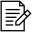
\includegraphics{./img/alg.png} Indica que el codi mostrat està en
\textbf{llenguatge algorísmic}.


\includegraphics{./img/c.png} Indica que el codi mostrat està en
\textbf{llenguatge C}.

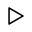
\includegraphics{./img/play.png} Mostra l'execució d'un programa en
\textbf{llenguatge C}.

\chapter{PAC01}\label{pac01}

\section{Llenguatge algorísmic}\label{llenguatge-algorismic}

El llenguatge algorísmic l'hem d'entendre com una aproximació al món
real, el qual utilitza unes normes definides per nosaltres mateixos. En
aquest punt encara no parlem de programes escrits en \textbf{C}, en
\textbf{Java}, en \textbf{Python} o en \textbf{PHP}, per dir alguns
llenguatges de programació.

Per exemple, en el llenguatge algorísmic que utilitzem a l'assignatura
definim un bloc de variables de la següent forma:

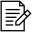
\includegraphics{./img/alg.png}

\begin{verbatim}
var
    edat: integer;
    pes: real;
end var
\end{verbatim}

Que es tracti d'un llenguatge més proper al món real no significa que no
s'hagin de complir unes determinades regles. Com es pot veure en aquest
exemple, una d'aquestes regles és que quan definim variables ho precedim
amb \texttt{var} i ho finalitzem amb \texttt{end\ var}.

Hem decidit utilitzar aquesta forma de llenguatge algorísmic, tot i que
també ho podríem haver plantejat de la següent forma :

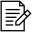
\includegraphics{./img/alg.png}

\begin{verbatim}
variable
    enter edat
    decimal pes
fvariable
\end{verbatim}

Remarcar que aquest segon exemple \textbf{és incorrecte}, no segueix la
nomenclatura del llenguatge algorísmic definit a l'assignatura. El
correcte és el primer exemple.

El llenguatge algorísmic és com fer una aproximació formal a la
realitat, no és un llenguatge de programació en sí com és \textbf{C},
\textbf{Java} o similars. Per tant no és un llenguatge que es pugui
compilar i executar amb l'IDE utilitzat a l'assignatura, el qual està
preparat únicament per interpretar i executar codi programat en
llenguatge C.

Ara bé la gran pregunta: i per què és necessari primer dissenyar
l'algorisme, si puc directament programar-ho en C?

Un algorisme ens permet dissenyar un programa sense tenir presents les
particularitats de cada llenguatge de programació. Aquesta aproximació
formal a la realitat dels algorismes ens faciliten poder fer
posteriorment una traducció ràpida a qualsevol llenguatge de programació
simplement coneixent les equivalències corresponents. Per exemple, el
primer cas si el programem en C equival a:


\includegraphics{./img/c.png}

\begin{Shaded}
\begin{Highlighting}[]
\DataTypeTok{int}\NormalTok{ edat;}
\DataTypeTok{float}\NormalTok{ pes;}
\end{Highlighting}
\end{Shaded}

El codi en C no el podem canviar, ja que si en comptes de posar int
utilitzem enter, el compilador de C no comprèn el mot i ens donarà un
error de codi.

Si mai hem programat és normal que aquest plantejament sobti al
principi, però és important que poc a poc es vagi veient les diferències
entre llenguatge algorísmic i llenguatge C.

\section{Llenguatge algorísmic vs llenguatge
C}\label{llenguatge-algorismic-vs-llenguatge-c}

En general:

\begin{itemize}
\tightlist
\item
  \textbf{Llenguatge algorísmic}: proper al llenguatge natural, es
  tracta d'una convenció que adoptem nosaltres mateixos per definir el
  un programa formalment. Els algorismes tenen una sèrie de normes i
  sentències que nosaltres definim (\textbf{Nomenclàtor}), però que no
  són de cap forma interpretables per un ordinador. Per tant un
  algorisme \textbf{no pot ser compilat ni executat}.
\item
  \textbf{Llenguatge C}: es tracta d'un llenguatge de programació que sí
  comprèn un ordinador. Això significa que únicament podem utilitzar les
  seves comandes i les seves normes per tal que el codi pugui ser
  compilat i executat sense problemes.
\end{itemize}

El llenguatge algorísmic és un pseudocodi que ens ajuda a definir com
funciona un programa. No està lligat a cap llenguatge de programació,
amb el que les accions que realitzarà, la forma de definir variables,
etc. és genèrica. Funcions com \texttt{writeString()},
\texttt{readInteger()} o \texttt{writeChar()} formen part del llenguatge
algorísmic: indiquen una acció genèrica a realitzar, com és escriure una
cadena de caracters, llegir un enter o escriure un caràcter. Quan es
vulgui codificar aquest algorisme en un llenguatge de programació
concret com és C, només caldrà saber les comandes pròpies de C que ens
permeten implementar l'algorisme.

La programació en C funciona exclusivament amb la sintaxi definida per
aquest llenguatge de programació. Instruccions com \texttt{scanf()} i
\texttt{printf()} són pròpies de C.

A mode d'exemple:

\textbf{Algorisme}: volem introduïr la lectura de la llum de casa
nostra; una possible implementació és:

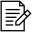
\includegraphics{./img/alg.png}

\begin{verbatim}
var
    lecturaMensual: integer;
end var

writeString("Introdueix la lectura mensual de la llum (kWh): ");
lecturaMensual := readInteger();
\end{verbatim}

\textbf{Llenguatge C}: en aquest llenguatge no existeixen les funcions
algorísmiques \texttt{writeString()} ni \texttt{readInteger()}, però en
canvi sí que tenim vàries funcions pròpies de C que ens permeten llegir
un valor per teclat i assignar-lo a una variable d'entorn. Per tant, les
accions algorísmiques anteriors correspondran a la següent codificació
en C:


\includegraphics{./img/c.png}

\begin{Shaded}
\begin{Highlighting}[]
\DataTypeTok{int}\NormalTok{ lecturaMensual;}

\NormalTok{printf(}\StringTok{"Introdueix la lectura mensual de la llum (kWh): "}\NormalTok{);}
\NormalTok{scanf(}\StringTok{"%d"}\NormalTok{, &lecturaMensual);}
\end{Highlighting}
\end{Shaded}

És molt important que es vegi clarament què és un algorisme i què és un
programa en C.

\section{Impressió de valors
incorrecta}\label{impressio-de-valors-incorrecta}

Quan es mostra per pantalla el contingut d'alguna variable amb
\texttt{printf()}, és important eliminar el prefix \texttt{\&} de la
variable:


\includegraphics{./img/c.png}

\begin{Shaded}
\begin{Highlighting}[]
\PreprocessorTok{#include }\ImportTok{<stdio.h>}

\DataTypeTok{int}\NormalTok{ main(}\DataTypeTok{int}\NormalTok{ argc, }\DataTypeTok{char}\NormalTok{ **argv)\{}

    \DataTypeTok{int}\NormalTok{ idAvio;}

\NormalTok{    printf(}\StringTok{"Introdueix l'identificador d'avió : "}\NormalTok{);}
\NormalTok{    scanf(}\StringTok{"%d"}\NormalTok{, &idAvio);}
    
\NormalTok{    printf(}\StringTok{">> Has escollit l'avió amb id %d }\SpecialCharTok{\textbackslash{}n}\StringTok{"}\NormalTok{, &idAvio);}

    \ControlFlowTok{return} \DecValTok{0}\NormalTok{;}
\NormalTok{\}}
\end{Highlighting}
\end{Shaded}

El resultat de l'execució és:


\includegraphics{./img/c.png}

\begin{Shaded}
\begin{Highlighting}[]
\NormalTok{Introdueix l'identificador d'avió : }\DecValTok{9}
\NormalTok{>> Has escollit l'avió amb id -}\DecValTok{1078693464}
\end{Highlighting}
\end{Shaded}

Quan fem referència a \texttt{\&idAvio} estem obtenint realment la
posició de memòria on resideix la variable \texttt{idAvio}. Per obtenir
el seu valor cal eliminar de dins \texttt{printf()} el prefix
\texttt{\&} de la variable \texttt{idAvio}:


\includegraphics{./img/c.png}

\begin{Shaded}
\begin{Highlighting}[]
\PreprocessorTok{#include }\ImportTok{<stdio.h>}

\DataTypeTok{int}\NormalTok{ main(}\DataTypeTok{int}\NormalTok{ argc, }\DataTypeTok{char}\NormalTok{ **argv)\{}

    \DataTypeTok{int}\NormalTok{ idAvio;}

\NormalTok{    printf(}\StringTok{"Introdueix l'identificador d'avió : "}\NormalTok{);}
\NormalTok{    scanf(}\StringTok{"%d"}\NormalTok{, &idAvio);}
    
\NormalTok{    printf(}\StringTok{">> Has escollit l'avió amb id %d }\SpecialCharTok{\textbackslash{}n}\StringTok{"}\NormalTok{, &idAvio);}

    \ControlFlowTok{return} \DecValTok{0}\NormalTok{;}
\NormalTok{\}}
\end{Highlighting}
\end{Shaded}

La sortida generada ara sí és correcta:

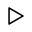
\includegraphics{./img/play.png}

\begin{Shaded}
\begin{Highlighting}[]
\NormalTok{Introdueix l'identificador d'avió : }\DecValTok{9}
\NormalTok{>> Has escollit l'avió amb id }\DecValTok{9} 
\end{Highlighting}
\end{Shaded}

\section{Com definir un enumeratiu}\label{com-definir-un-enumeratiu}

La definició d'un tipus enumeratiu es fa de la següent forma:

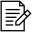
\includegraphics{./img/alg.png}

\begin{verbatim}
type
    typeName = {VALUE1, VALUE2, VALUE3, ... , VALUEn};
end type
\end{verbatim}

Els elements \texttt{VALUE1}, \texttt{VALUE2}, \texttt{VALUE3}\ldots{}
acaben sent constants, i el valor que de cadascun és:

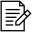
\includegraphics{./img/alg.png}

\begin{verbatim}
VALUE1 = 0
VALUE2 = 1
VALUE3 = 2 
{ ... }
VALUEn = n-1
\end{verbatim}

Posteriorment no és possible fer un canvi de valor d'aquests elements de
tipus enumeratiu.

\section{Com utilitzar un enumeratiu}\label{com-utilitzar-un-enumeratiu}

Una enumeració simplement és una assignació d'un valor enter, començant
pel 0 i incrementant-se en 1, a la sèrie d'elements que l'hi has
definit.

Per exemple, podem tenir la següent definició:


\includegraphics{./img/c.png}

\begin{Shaded}
\begin{Highlighting}[]
\KeywordTok{typedef} \KeywordTok{enum}\NormalTok{ \{MALE, FEMALE\} tGender;}
\end{Highlighting}
\end{Shaded}

Això significa que internament \texttt{MALE\ ==\ 0} i
\texttt{FEMALE\ ==\ 1}. Si l'ordre de la definició l'haguessis fet al
revés, \texttt{\{FEMALE,\ MALE\}}, tindríem que \texttt{FEMALE\ ==\ 0} i
\texttt{MALE\ ==\ 1}.

D'aquesta forma es llegeix un enter i es compara el seu valor amb un o
altre element de l'\texttt{enum} per tal de fer l'acció que desitgem.
Una possible implementació en llenguatge C seria:


\includegraphics{./img/c.png}

\begin{Shaded}
\begin{Highlighting}[]
\PreprocessorTok{#include }\ImportTok{<stdio.h>}

\DataTypeTok{int}\NormalTok{ main(}\DataTypeTok{int}\NormalTok{ argc, }\DataTypeTok{char}\NormalTok{ **argv) \{}

   \KeywordTok{typedef} \KeywordTok{enum}\NormalTok{ \{MALE, FEMALE\} tGender;}

\NormalTok{   tGender gender;}

\NormalTok{   printf(}\StringTok{"Type patient gender: 0 for MALE, 1 for FEMALE}\SpecialCharTok{\textbackslash{}n}\StringTok{"}\NormalTok{);}
\NormalTok{   scanf(}\StringTok{"%d"}\NormalTok{, &gender);}

   \ControlFlowTok{if}\NormalTok{ (gender == MALE) \{}
\NormalTok{      printf(}\StringTok{"Patient gender MALE}\SpecialCharTok{\textbackslash{}n}\StringTok{"}\NormalTok{);}
\NormalTok{   \} }\ControlFlowTok{else}\NormalTok{ \{}
      \ControlFlowTok{if}\NormalTok{ (gender == FEMALE) \{}
\NormalTok{         printf(}\StringTok{"Patient gender FEMALE}\SpecialCharTok{\textbackslash{}n}\StringTok{"}\NormalTok{);}
\NormalTok{      \} }\ControlFlowTok{else}\NormalTok{ \{}
\NormalTok{         printf(}\StringTok{"Incorrect option}\SpecialCharTok{\textbackslash{}n}\StringTok{"}\NormalTok{);}
\NormalTok{      \}}
\NormalTok{   \}}
\NormalTok{\}}
\end{Highlighting}
\end{Shaded}

\section{Especificador d'un
enumeratiu}\label{especificador-dun-enumeratiu}

Els enumeratius en llenguatge C, \texttt{enum}, utilitzen
l'especificador \texttt{\%u} independentment del tipus que s'hagi
definit per l'enumeratiu.

Exemple:


\includegraphics{./img/c.png}

\begin{Shaded}
\begin{Highlighting}[]
\PreprocessorTok{#include }\ImportTok{<stdio.h>}

\KeywordTok{typedef} \KeywordTok{enum}\NormalTok{ \{PRIVAT, PUBLIC\} tTransport;}

\DataTypeTok{int}\NormalTok{ main(}\DataTypeTok{int}\NormalTok{ argc, }\DataTypeTok{char}\NormalTok{ **argv) \{}
\NormalTok{    tTransport tipusTransport;}

\NormalTok{    printf(}\StringTok{"Com et desplaces a la feina (0=privat, 1=públic) ? : "}\NormalTok{);}
\NormalTok{    scanf(}\StringTok{"%u"}\NormalTok{, &tipusTransport);}
\NormalTok{    printf(}\StringTok{"Et desplaces a la feina amb transport (0=privat, 1=públic) : "}\NormalTok{);}
\NormalTok{    printf(}\StringTok{"%u}\SpecialCharTok{\textbackslash{}n}\StringTok{"}\NormalTok{, tipusTransport);}
\NormalTok{\}}
\end{Highlighting}
\end{Shaded}

\section{Lectura de caràcters en C}\label{lectura-de-caracters-en-c}

En el llenguatge C la lectura d'un \texttt{char} pot comportar-se de
forma inadequada si prèviament el buffer d'entrada conté algun caràcter
previ.

Imaginem que volem crear un programa molt senzill que donat un número de
DNI i la seva lletra, ens concateni els dos valors i ho mostri per
pantalla. Una possible forma d'implementar aquest programa en C seria:


\includegraphics{./img/c.png}

\begin{Shaded}
\begin{Highlighting}[]
\PreprocessorTok{#include }\ImportTok{<stdio.h>}

\DataTypeTok{int}\NormalTok{ main(}\DataTypeTok{int}\NormalTok{ argc, }\DataTypeTok{char}\NormalTok{ **argv) \{}

    \DataTypeTok{int}\NormalTok{ dniNum;   }\CommentTok{/* número del DNI */}
    \DataTypeTok{char}\NormalTok{ dniChar; }\CommentTok{/* lletra del DNI */}

\NormalTok{    printf(}\StringTok{"Introdueix el número del DNI: "}\NormalTok{);}
\NormalTok{    scanf(}\StringTok{"%d"}\NormalTok{, &dniNum);}
\NormalTok{    printf(}\StringTok{"Introdueix la lletra del DNI: "}\NormalTok{);}
\NormalTok{    scanf(}\StringTok{"%c"}\NormalTok{, &dniChar);}

\NormalTok{    printf(}\StringTok{"}\SpecialCharTok{\textbackslash{}n}\StringTok{El DNI introduit és: %d-%c}\SpecialCharTok{\textbackslash{}n}\StringTok{"}\NormalTok{, dniNum, dniChar);}

    \ControlFlowTok{return} \DecValTok{0}\NormalTok{;}
\NormalTok{\}}
\end{Highlighting}
\end{Shaded}

Què passa si executem aquest codi? Que veiem que es comporta de forma
incorrecta, ja que no ens arriba a demanar la lletra del DNI, mostrant
directament el resultat:

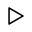
\includegraphics{./img/play.png}

\begin{Shaded}
\begin{Highlighting}[]
\NormalTok{Introdueix el número del DNI: }\DecValTok{12345678}
\NormalTok{Introdueix la lletra del DNI:}
\NormalTok{El DNI introduit és: }\DecValTok{12345678}\NormalTok{-}
\end{Highlighting}
\end{Shaded}

Quan teclegem el primer enter el que fem realment és introduir un número
+ un \texttt{intro} al final de tot. El número queda assignat a la
variable \texttt{dni\_num}, i l'\texttt{intro} és llegit com un caràcter
i s'assigna a la variable \texttt{dni\_char}. Per aquest motiu C
interpreta que les dues variables ja tenen valor i finalitza el
programa.

Com podem solucionar aquest comportament? Buidant l'\texttt{intro} del
buffer d'entrada abans de llegir el caràcter, i això ho podem fer amb la
comanda \texttt{getchar()}. Aquesta comanda llegeix un caràcter del
buffer d'entrada i el buida del buffer.

Per tant es pot corregir el programa anterior de la següent forma:


\includegraphics{./img/c.png}

\begin{Shaded}
\begin{Highlighting}[]
\PreprocessorTok{#include }\ImportTok{<stdio.h>}

\DataTypeTok{int}\NormalTok{ main(}\DataTypeTok{int}\NormalTok{ argc, }\DataTypeTok{char}\NormalTok{ **argv) \{}

    \DataTypeTok{int}\NormalTok{ dni_num; }\CommentTok{// número del DNI}
    \DataTypeTok{char}\NormalTok{ dni_char; }\CommentTok{// lletra del DNI}

\NormalTok{    printf(}\StringTok{"Introdueix el número del DNI: "}\NormalTok{);}
\NormalTok{    scanf(}\StringTok{"%d"}\NormalTok{, &dni_num);}
\NormalTok{    getchar();}
\NormalTok{    printf(}\StringTok{"Introdueix la lletra del DNI: "}\NormalTok{);}
\NormalTok{    scanf(}\StringTok{"%c"}\NormalTok{, &dni_char);}

\NormalTok{    printf(}\StringTok{"}\SpecialCharTok{\textbackslash{}n}\StringTok{El DNI introduit és: %d-%c}\SpecialCharTok{\textbackslash{}n}\StringTok{"}\NormalTok{, dni_num, dni_char);}

    \ControlFlowTok{return} \DecValTok{0}\NormalTok{;}
\NormalTok{\}}
\end{Highlighting}
\end{Shaded}

Si ara executem, ja funcionarà com desitgem:

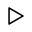
\includegraphics{./img/play.png}

\begin{Shaded}
\begin{Highlighting}[]
\NormalTok{Introdueix el número del DNI: }\DecValTok{12345678}
\NormalTok{Introdueix la lletra del DNI: B}

\NormalTok{El DNI introduit és: }\DecValTok{12345678}\NormalTok{-B}
\end{Highlighting}
\end{Shaded}

En cas de necessitat, amb \texttt{getChar()} es pot guardar el caràcter
del buffer en una variable, per tal de tractar-lo posteriorment:


\includegraphics{./img/c.png}

\begin{Shaded}
\begin{Highlighting}[]
\DataTypeTok{char}\NormalTok{ nomVariable;}
\NormalTok{nomVariable = getChar();}
\end{Highlighting}
\end{Shaded}

\section{Lectura de float en C}\label{lectura-de-float-en-c}

El separador de valors decimals (tipus \texttt{float}) en C \textbf{és
el punt}, no la coma. Per aquest motiu quan s'introdueix un valor
decimal des de teclat, sempre ho farem amb un punt:

Exemple:


\includegraphics{./img/c.png}

\begin{Shaded}
\begin{Highlighting}[]
\PreprocessorTok{#include }\ImportTok{<stdio.h>}

\DataTypeTok{int}\NormalTok{ main(}\DataTypeTok{int}\NormalTok{ argc, }\DataTypeTok{char}\NormalTok{ **argv) \{\}}

    \CommentTok{/* Variable que contindrà el pes d’una persona */}
    \DataTypeTok{float}\NormalTok{ pes;}

    \CommentTok{/* Lectura de la dada per teclat (el separador de decimals és un . ) */}
\NormalTok{    printf(}\StringTok{"Introdueix el pes (kg) d’una persona : "}\NormalTok{);}
\NormalTok{    scanf(}\StringTok{"%f"}\NormalTok{, &pes);}

   \CommentTok{/* Es mostra el valor decimal per pantalla */}
\NormalTok{   printf(}\StringTok{"Has introduit el pes = %.1f kg.}\SpecialCharTok{\textbackslash{}n}\StringTok{"}\NormalTok{, pes);}

   \ControlFlowTok{return} \DecValTok{0}\NormalTok{;}
\NormalTok{\}}
\end{Highlighting}
\end{Shaded}

L'execució serà:

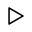
\includegraphics{./img/play.png}

\begin{Shaded}
\begin{Highlighting}[]
\NormalTok{Introdueix el pes (kg) d’una persona : }\FloatTok{79.440}
\NormalTok{Has introduit el pes = }\FloatTok{79.4}\NormalTok{ kg.}
\end{Highlighting}
\end{Shaded}

\chapter{PAC02}\label{pac02}

\section{define vs const}\label{define-vs-const}

La definició de constants tant es pot fer amb \texttt{define} com amb
\texttt{const}. Tot i això, la forma de comportar-se d'aquestes dues
opcions és completament diferent, si ve el resultat final és el mateix:

\begin{itemize}
\tightlist
\item
  \texttt{define}: quan utilitzem aquesta opció no es desa en cap
  posició de memòria el valor de la constant. El que es fa realment és
  que en els passos previs a la pròpia compilació del programa, el
  preprocessador substitueix totes les referencies del define pel valor
  indicat.
\end{itemize}

Per exemple, si tenim el següent programa amb una constant creada amb
\texttt{define} :


\includegraphics{./img/c.png}

\begin{Shaded}
\begin{Highlighting}[]
\PreprocessorTok{#include }\ImportTok{<stdio.h>}
\PreprocessorTok{#define MIDA 8}

\DataTypeTok{char}\NormalTok{ lletres[] = \{}\CharTok{'a'}\NormalTok{, }\CharTok{'b'}\NormalTok{, }\CharTok{'c'}\NormalTok{, }\CharTok{'d'}\NormalTok{, }\CharTok{'e'}\NormalTok{, }\CharTok{'f'}\NormalTok{, }\CharTok{'g'}\NormalTok{, }\CharTok{'h'}\NormalTok{\};}
\DataTypeTok{int}\NormalTok{ vertical, horitzontal;}

\DataTypeTok{int}\NormalTok{ main(}\DataTypeTok{int}\NormalTok{ argc, }\DataTypeTok{char}\NormalTok{ **argv) \{}
    \CommentTok{/* font: https://en.wikipedia.org/wiki/Chess */}

    \ControlFlowTok{for}\NormalTok{ (vertical=MIDA; vertical>=}\DecValTok{1}\NormalTok{; vertical--) \{}
        \ControlFlowTok{for}\NormalTok{ (horitzontal=}\DecValTok{0}\NormalTok{; horitzontal<=MIDA-}\DecValTok{1}\NormalTok{; horitzontal++) \{}
\NormalTok{            printf(}\StringTok{"%c%d "}\NormalTok{, lletres[horitzontal], vertical);}
\NormalTok{        \}}
\NormalTok{        printf(}\StringTok{"}\SpecialCharTok{\textbackslash{}n}\StringTok{"}\NormalTok{);}
\NormalTok{    \}}
\NormalTok{\}}
\end{Highlighting}
\end{Shaded}

Abans de la compilació, el preprocessador entre altres accions elimina
comentaris i substitueix totes les referències \texttt{MIDA} per
\texttt{8}:


\includegraphics{./img/c.png}

\begin{Shaded}
\begin{Highlighting}[]
\PreprocessorTok{#include }\ImportTok{<stdio.h>}

\DataTypeTok{char}\NormalTok{ lletres[] = \{}\CharTok{'a'}\NormalTok{, }\CharTok{'b'}\NormalTok{, }\CharTok{'c'}\NormalTok{, }\CharTok{'d'}\NormalTok{, }\CharTok{'e'}\NormalTok{, }\CharTok{'f'}\NormalTok{, }\CharTok{'g'}\NormalTok{, }\CharTok{'h'}\NormalTok{\};}
\DataTypeTok{int}\NormalTok{ vertical, horitzontal;}

\DataTypeTok{int}\NormalTok{ main(}\DataTypeTok{int}\NormalTok{ argc, }\DataTypeTok{char}\NormalTok{ **argv) \{}

    \ControlFlowTok{for}\NormalTok{ (vertical=}\DecValTok{8}\NormalTok{; vertical>=}\DecValTok{1}\NormalTok{; vertical--) \{}
        \ControlFlowTok{for}\NormalTok{ (horitzontal=}\DecValTok{0}\NormalTok{; horitzontal<=}\DecValTok{8}\NormalTok{-}\DecValTok{1}\NormalTok{; horitzontal++) \{}
\NormalTok{            printf(}\StringTok{"%c%d "}\NormalTok{, lletres[horitzontal], vertical);}
\NormalTok{        \}}
\NormalTok{        printf(}\StringTok{"}\SpecialCharTok{\textbackslash{}n}\StringTok{"}\NormalTok{);}
\NormalTok{    \}}
\NormalTok{\}}
\end{Highlighting}
\end{Shaded}

Per tant la definició de constants amb \texttt{define} es comporta com
si d'un ``cercar-reemplaçar'' d'un processador de textos es tractés. No
es desa cap constant en memòria, però per contra, el programa ocuparà
una mica més per la substitució directa de referències que fa; la
substitució la fa en tot el programa, no es pot limitar a un àmbit
concret (per exemple només dins d'una funció).

\begin{itemize}
\tightlist
\item
  \texttt{const}: en aquest cas sí que es reserva una posició de
  memòria. En C es comporta igual com si fos una variable, però la qual
  únicament funciona en mode lectura: no li podem modificar el valor.
\end{itemize}

A més, \texttt{const} ens permet també dir quin tipus de valor tindrà la
constant: si és de tipus \texttt{float}, \texttt{int},
\texttt{char}\ldots{} amb el que aquest fet ens dóna un punt addicional
de control, ja que ens assegurem que el tipus de valor assignat serà el
correcte pel programa.

Amb aquest tipus de definició de constant, l'exemple anterior quedaria
de la següent forma:


\includegraphics{./img/c.png}

\begin{Shaded}
\begin{Highlighting}[]
\PreprocessorTok{#include }\ImportTok{<stdio.h>}
\DataTypeTok{const} \DataTypeTok{int}\NormalTok{ MIDA }\DecValTok{8}

\DataTypeTok{char}\NormalTok{ lletres[] = \{}\CharTok{'a'}\NormalTok{, }\CharTok{'b'}\NormalTok{, }\CharTok{'c'}\NormalTok{, }\CharTok{'d'}\NormalTok{, }\CharTok{'e'}\NormalTok{, }\CharTok{'f'}\NormalTok{, }\CharTok{'g'}\NormalTok{, }\CharTok{'h'}\NormalTok{\};}
\DataTypeTok{int}\NormalTok{ vertical, horitzontal;}

\DataTypeTok{int}\NormalTok{ main(}\DataTypeTok{int}\NormalTok{ argc, }\DataTypeTok{char}\NormalTok{ **argv) \{}

    \CommentTok{/* La constant MIDA està desada en memòria */}
\NormalTok{    printf(}\StringTok{"posició en memòria de la constant MIDA : %p }\SpecialCharTok{\textbackslash{}n}\StringTok{"}\NormalTok{, &MIDA);}

    \ControlFlowTok{for}\NormalTok{ (vertical=MIDA; vertical>=}\DecValTok{1}\NormalTok{; vertical--) \{}
        \ControlFlowTok{for}\NormalTok{ (horitzontal=}\DecValTok{0}\NormalTok{; horitzontal<=MIDA-}\DecValTok{1}\NormalTok{; horitzontal++) \{}
\NormalTok{            printf(}\StringTok{"%c%d "}\NormalTok{, lletres[horitzontal], vertical);}
\NormalTok{        \}}
\NormalTok{        printf(}\StringTok{"}\SpecialCharTok{\textbackslash{}n}\StringTok{"}\NormalTok{);}
\NormalTok{    \}}
\NormalTok{\}}
\end{Highlighting}
\end{Shaded}

Com es pot veure, és possible obtinir l'adreça en memòria on es desa la
constant \texttt{MIDA}. En aquest cas, sí que pots definir una constant
amb \texttt{const} i fer que només afecti un àmbit determinat (per
exemple, que la constant estigui definida únicament dins d'una funció).

Aquestes són les principals diferències entre \texttt{define} i
\texttt{const} a l'hora de definir una constant; \texttt{define} es va
crear molt abans que no la sentència \texttt{const}, amb el que és un
habit força habitual decantar-se per aquesta opció per temes més
històrics.

\section{Precisió en variables float}\label{precisio-en-variables-float}

Hi ha alguns valors decimals determinats que no es poden representar de
forma precisa en una variable de tipus \texttt{float}. La millor solució
pels casos que tractem és arrodonir al número de decimals que realment
necessitem.

Si en canvi volem sí o sí treballar amb tots els decimals, podem optar
per utilitzar un tipus de dada que tingui major precisió que
\texttt{float}: \texttt{double}.

Per exemple, el següent programa retorna el resultat esperat si es desa
en un \texttt{double}, i no així si es fa en un \texttt{float}:


\includegraphics{./img/c.png}

\begin{Shaded}
\begin{Highlighting}[]
\PreprocessorTok{#include }\ImportTok{<stdio.h>}

\DataTypeTok{int}\NormalTok{ main() \{ }

    \DataTypeTok{float}\NormalTok{ num1; }
    \DataTypeTok{float}\NormalTok{ num2;}
    \DataTypeTok{float}\NormalTok{ resultat1; }
    \DataTypeTok{double}\NormalTok{ resultat2; }
    
\NormalTok{    num1 = }\FloatTok{1.3}\NormalTok{; }
\NormalTok{    num2 = }\DecValTok{17}\NormalTok{;}
\NormalTok{    resultat1 = num1 + num2; }
\NormalTok{    printf(}\StringTok{"resultat amb float: %f}\SpecialCharTok{\textbackslash{}n}\StringTok{"}\NormalTok{, resultat1); }
\NormalTok{    resultat2 = num1 + num2; }
\NormalTok{    printf(}\StringTok{"resultat amb double: %f}\SpecialCharTok{\textbackslash{}n}\StringTok{"}\NormalTok{, resultat2); }
    \ControlFlowTok{return} \DecValTok{0}\NormalTok{; }
\NormalTok{\}}
\end{Highlighting}
\end{Shaded}

La sortida que genera és:

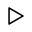
\includegraphics{./img/play.png}

\begin{Shaded}
\begin{Highlighting}[]
\NormalTok{resultat amb  }\DataTypeTok{float}\NormalTok{: }\FloatTok{18.299999}
\NormalTok{resultat amb }\DataTypeTok{double}\NormalTok{: }\FloatTok{18.300000}
\end{Highlighting}
\end{Shaded}

\section{Expressions}\label{expressions}

\subsection{Exemple 1: esParell}\label{exemple-1-esparell}

Imaginem que ens demanen un algorisme que indiqui si un número és
parell.

Una possible solució seria:

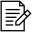
\includegraphics{./img/alg.png}

\begin{verbatim}
algorithm esParell
    var
        numero: integer;
        isParell: boolean;
    end var

    writeString("Introdueix un número : ");
    numero:= readInteger();
    isParell:= (numero mod 2 = 0);
    
    writeString("El numero ");
    writeInteger(numero);
    writeString(" és parell? ");
    writeBoolean(isParell);

end algorithm
\end{verbatim}

La variable \texttt{isParell} prendrà el valor \texttt{TRUE} si el
número es parell i \texttt{FALSE} en cas contrari. No ha calgut
utilitzar cap estructura \texttt{if-else} per resoldre l'algorisme.

Una possible forma de codificar-ho en llenguatge C és:


\includegraphics{./img/c.png}

\begin{Shaded}
\begin{Highlighting}[]
\PreprocessorTok{#include }\ImportTok{<stdio.h>}

\KeywordTok{typedef} \KeywordTok{enum}\NormalTok{ \{FALSE, TRUE\} boolean;}

\DataTypeTok{int}\NormalTok{ main(}\DataTypeTok{int}\NormalTok{ argc, }\DataTypeTok{char}\NormalTok{ **argv) \{}

    \DataTypeTok{int}\NormalTok{ numero;}
\NormalTok{    boolean isParell;}

\NormalTok{    printf(}\StringTok{"Introdueix un número : "}\NormalTok{);}
\NormalTok{    scanf(}\StringTok{"%d"}\NormalTok{, &numero);}
\NormalTok{    isParell = (numero % }\DecValTok{2}\NormalTok{ == }\DecValTok{0}\NormalTok{);}
    
\NormalTok{    printf(}\StringTok{"El número %d és parell? (0=FALSE, 1=TRUE) : %u }\SpecialCharTok{\textbackslash{}n}\StringTok{"}\NormalTok{, numero, isParell);}

    \ControlFlowTok{return} \DecValTok{0}\NormalTok{;}
\NormalTok{\}}
\end{Highlighting}
\end{Shaded}

\subsection{Exemple 2: capDeSetmana}\label{exemple-2-capdesetmana}

Imaginem que volem fer un programa molt senzill que ens digui si avui és
cap de setmana o no. El seu algorisme seria el següent:

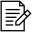
\includegraphics{./img/alg.png}

\begin{verbatim}
type
    dies = {DILLUNS, DIMARTS, DIMECRES, DIJOUS, DIVENDRES, DISSABTE, DIUMENGE};
end type

algorithm capDeSetmana

    var
        esCapDeSetmana: boolean;
        diaSetmana: dies;
    end var

    writeString("Quin dia de la setmana és avui ?\n");
    writeString("Per DILLUNS tecleja 0\n");
    writeString("Per DIMARTS tecleja 1\n");
    writeString("Per DIMECRES tecleja 2\n");
    writeString("Per DIJOUS tecleja 3\n");
    writeString("Per DIVENDRES tecleja 4\n");
    writeString("Per DISSABTE tecleja 5\n");
    writeString("Per DIUMENGE tecleja 6\n");
 
    diaSetmana:= readInteger();
    esCapDeSetmana:= (diaSetmana = DISSABTE or diaSetmana = DIUMENGE);

    writeString("Avui és cap de setmana?");
    writeBool(esCapDeSetmana);

end algorithm
\end{verbatim}

La variable \texttt{boolean} \texttt{esCapDeSetmana} prendrà el valor de
\texttt{TRUE} o \texttt{FALSE} en funció del resultat d'avaluar
l'expressió. No és necessari la utilització d'estructures condicionals
\texttt{if-else} que veurem més endavant en el curs.

Una possible forma de codificar-ho en llenguatge C és:


\includegraphics{./img/c.png}

\begin{Shaded}
\begin{Highlighting}[]
\PreprocessorTok{#include }\ImportTok{<stdio.h>}

\KeywordTok{typedef} \KeywordTok{enum}\NormalTok{ \{FALSE, TRUE\} boolean;}
\KeywordTok{typedef} \KeywordTok{enum}\NormalTok{ \{DILLUNS, DIMARTS, DIMECRES, DIJOUS, DIVENDRES, DISSABTE, DIUMENGE\} dies;}

\DataTypeTok{int}\NormalTok{ main(}\DataTypeTok{int}\NormalTok{ argc, }\DataTypeTok{char}\NormalTok{ **argv) \{}

\NormalTok{    boolean esCapDeSetmana;}
\NormalTok{    dies diaSetmana;}

\NormalTok{    printf(}\StringTok{"}\SpecialCharTok{\textbackslash{}n}\StringTok{Quin dia de la setmana és avui ?}\SpecialCharTok{\textbackslash{}n}\StringTok{"}\NormalTok{);}
\NormalTok{    printf(}\StringTok{"Per DILLUNS tecleja 0}\SpecialCharTok{\textbackslash{}n}\StringTok{"}\NormalTok{);}
\NormalTok{    printf(}\StringTok{"Per DIMARTS tecleja 1}\SpecialCharTok{\textbackslash{}n}\StringTok{"}\NormalTok{);}
\NormalTok{    printf(}\StringTok{"Per DIMECRES tecleja 2}\SpecialCharTok{\textbackslash{}n}\StringTok{"}\NormalTok{);}
\NormalTok{    printf(}\StringTok{"Per DIJOUS tecleja 3}\SpecialCharTok{\textbackslash{}n}\StringTok{"}\NormalTok{);}
\NormalTok{    printf(}\StringTok{"Per DIVENDRES tecleja 4}\SpecialCharTok{\textbackslash{}n}\StringTok{"}\NormalTok{);}
\NormalTok{    printf(}\StringTok{"Per DISSABTE tecleja 5}\SpecialCharTok{\textbackslash{}n}\StringTok{"}\NormalTok{);}
\NormalTok{    printf(}\StringTok{"Per DIUMENGE tecleja 6}\SpecialCharTok{\textbackslash{}n}\StringTok{"}\NormalTok{);}

\NormalTok{    scanf(}\StringTok{"%u"}\NormalTok{, &diaSetmana);}
\NormalTok{    esCapDeSetmana = (diaSetmana == DISSABTE || diaSetmana == DIUMENGE);}

\NormalTok{    printf(}\StringTok{"Avui és cap de setmana (0 == FALSE, 1 == TRUE) ? %u}\SpecialCharTok{\textbackslash{}n}\StringTok{"}\NormalTok{, esCapDeSetmana);}

    \ControlFlowTok{return} \DecValTok{0}\NormalTok{;}
\NormalTok{\}}
\end{Highlighting}
\end{Shaded}

Varis punts a considerar:

\begin{itemize}
\tightlist
\item
  Recordem que en C no hi ha el tipus primitiu \texttt{boolean}, al
  mateix nivell que existeix un \texttt{int}, un \texttt{float} o un
  \texttt{char}\ldots{} Per tant definirem sempre el tipus
  \texttt{boolean} com un \texttt{enum} amb els components
  \texttt{\{FALSE,\ TRUE\}}.
\item
  Quan definim una variable de tipus \texttt{enum}, la
  llegirem/escriurem com a \texttt{\%u}. Ho podríem fer com a
  \texttt{\%d}, però us retornarà un warning tot i que el resultat sigui
  correcte. El tipus \texttt{\%u} és igual que un enter \texttt{\%d}
  però sense signe: això significa que amb \texttt{\%d} podem tractar
  valors negatius com -12 i amb \texttt{\%u} això no és possible, però
  com que sabem que els valors que pot prendre un \texttt{enum} sempre
  seran \textgreater{}= 0, ens convé utilitzar \texttt{\%u}.
\item
  Per les particularitats dels \texttt{boolean} en el llenguatge de
  programació C que ja hem comentat abans, l'entrada i sortida de valors
  d'un \texttt{boolean} serà numèrica. Per facilitar la comprensió podem
  mostrar per pantalla un literal que ens indiqui que 0 equival a
  \texttt{FALSE} i 1 a \texttt{TRUE}.

  \begin{itemize}
  \tightlist
  \item
    L'assignació de valors en els algorismes la fem amb \texttt{:=},
    però en llenguatge C es fa amb \texttt{=}.
  \item
    La comparació en els algorismes la fem amb \texttt{=}, però en
    llenguatge C es fa amb \texttt{==}.
  \item
    L'operació lògica \texttt{or} dels algorismes es tradueix en C amb
    l'operand \texttt{\textbar{}\textbar{}}.
  \item
    L'operació lògica \texttt{and} dels algorismes es tradueix en C amb
    l'operand \texttt{\&\&}.
  \end{itemize}
\end{itemize}

\subsection{Exemple 3:
ginTonicPreparation}\label{exemple-3-gintonicpreparation}

Imaginem que volem preparar un gintònic. Sabem el volum de ginebra i de
tònica que utilitzarem, i quina és la capacitat de la copa de baló que
el contindrà.

Hem vist una oferta per internet i hem comprat glaçons metàl·lics d'acer
inoxidable\ldots{} però se'ns ha anat una mica el cap i n'hem comprat un
total de 20 unitats.

Volem fer un programa que, utilitzant únicament expressions, ens digui
si podem preparar o no el gintònic en funció del número de glaçons que
li volem posar:

\begin{itemize}
\tightlist
\item
  si el nombre de glaçons caben dins de la copa, retornarà
  \texttt{true}.
\item
  en cas contrari, retornarà \texttt{false}.
\end{itemize}

Per tant el que ha de fer el nostre programa bàsicament és validar si el
volum de ginebra + tònica + (glaço) * número de glaçons supera o no el
volum de la copa.

L'algorisme podria ser el següent:

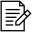
\includegraphics{./img/alg.png}

\begin{verbatim}
const
    GIN: real = 50.0;              { in ml }
    TONIC: real = 200.0;           { in ml }
    GLASS: real = 620.0;           { in ml }
    METAL_ICE_CUBE: real = 42.875; { in ml }
end const

algorithm ginTonicPreparation

    var
        numMetalIceCubes: integer;
        isPossible: boolean;
    end var

    writeString("Number of metal ice cubes ? (integer) : ");
    numMetalIceCubes:= readInteger();

    isPossible:= (GLASS ≥ (GIN + TONIC + METAL_ICE_CUBE * numMetalIceCubes));

    writeString("Can you make a gin & tonic? : ");
    writeBoolean(isPossible);

end algorithm
\end{verbatim}

L'expressió que dóna valor a \texttt{isPossible} s'ocupa d'avaluar el
volum de la copa respecte el resultant de ginebra, tònica i glaçons.

La seva traducció a C podria ser:


\includegraphics{./img/c.png}

\begin{Shaded}
\begin{Highlighting}[]
\PreprocessorTok{#include }\ImportTok{<stdio.h>}

\PreprocessorTok{#define GIN 50.0              }\CommentTok{/* in ml */}
\PreprocessorTok{#define TONIC 200.0           }\CommentTok{/* in ml */}
\PreprocessorTok{#define GLASS 620.0           }\CommentTok{/* in ml */}
\PreprocessorTok{#define METAL_ICE_CUBE 42.875 }\CommentTok{/* in ml */}\PreprocessorTok{ }

\KeywordTok{typedef} \KeywordTok{enum}\NormalTok{ \{FALSE, TRUE\} boolean;}

\DataTypeTok{int}\NormalTok{ main(}\DataTypeTok{int}\NormalTok{ argc, }\DataTypeTok{char}\NormalTok{ **argv) \{}

    \DataTypeTok{int}\NormalTok{ numMetalIceCubes;}
\NormalTok{    boolean isPossible;}

\NormalTok{    printf(}\StringTok{"Number of metal ice cubes ? (integer) : "}\NormalTok{);}
\NormalTok{    scanf(}\StringTok{"%d"}\NormalTok{, &numMetalIceCubes);}

\NormalTok{    isPossible = GLASS >= (GIN + TONIC + METAL_ICE_CUBE * numMetalIceCubes);}

\NormalTok{    printf(}\StringTok{"Can you make a gin & tonic? (0=FALSE, 1=TRUE) : %u}\SpecialCharTok{\textbackslash{}n}\StringTok{"}\NormalTok{, isPossible);}
    
    \ControlFlowTok{return} \DecValTok{0}\NormalTok{;}
\NormalTok{\}}
\end{Highlighting}
\end{Shaded}

Per realitzar el càlcul en C també s'ha utilitzat una expressió.

\subsection{Exemple 4: ginTonicFreeMl}\label{exemple-4-gintonicfreeml}

Anem a evolucionar l'exemple anterior del gintònic: imaginem ara que
volem que el nostre programa ens digui el volum (en mililitres) que
queda lliure a la copa una vegada posat un determinat nombre de glaçons.

L'algorisme quedaria de la següent forma:

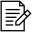
\includegraphics{./img/alg.png}

\begin{verbatim}
const
    GIN: real = 50.0;              { in ml }
    TONIC: real = 200.0;           { in ml }
    GLASS: real = 620.0;           { in ml }
    METAL_ICE_CUBE: real = 42.875; { in ml }
end const

algorithm ginTonicFreeMl

    var
        numMetalIceCubes: integer;
        volumeFree: real;
    end var

    writeString("Number of metal ice cubes ? (integer) : ");
    numMetalIceCubes:= readInteger();

    volumeFree:= GLASS - (GIN + TONIC + METAL_ICE_CUBE * numMetalIceCubes);

    writeString("How many free ml in the glass? : ");
    writeReal(volumeFree);

end algorithm
\end{verbatim}

I la codificació en C :


\includegraphics{./img/c.png}

\begin{Shaded}
\begin{Highlighting}[]
\PreprocessorTok{#include }\ImportTok{<stdio.h>}

\PreprocessorTok{#define GIN 50.0              }\CommentTok{/* in ml */}
\PreprocessorTok{#define TONIC 200.0           }\CommentTok{/* in ml */}
\PreprocessorTok{#define GLASS 620.0           }\CommentTok{/* in ml */}
\PreprocessorTok{#define METAL_ICE_CUBE 42.875 }\CommentTok{/* in ml */}

\KeywordTok{typedef} \KeywordTok{enum}\NormalTok{ \{FALSE, TRUE\} boolean;}

\DataTypeTok{int}\NormalTok{ main(}\DataTypeTok{int}\NormalTok{ argc, }\DataTypeTok{char}\NormalTok{ **argv) \{}

    \DataTypeTok{int}\NormalTok{ numMetalIceCubes;}
    \DataTypeTok{float}\NormalTok{ volumeFree;}

\NormalTok{    printf(}\StringTok{"Number of metal ice cubes ? (integer) : "}\NormalTok{);}
\NormalTok{    scanf(}\StringTok{"%d"}\NormalTok{, &numMetalIceCubes);}

\NormalTok{    volumeFree = GLASS - (GIN + TONIC + METAL_ICE_CUBE * numMetalIceCubes);}

\NormalTok{    printf(}\StringTok{"How many free ml in the glass ? : %.3f ml }\SpecialCharTok{\textbackslash{}n}\StringTok{"}\NormalTok{, volumeFree);}
    
    \ControlFlowTok{return} \DecValTok{0}\NormalTok{;}
\NormalTok{\}}
\end{Highlighting}
\end{Shaded}

\subsection{Exemple 5: scoutingBasquet}\label{exemple-5-scoutingbasquet}

Imaginem que fem tasques d'scouting per les seccions de bàsquet femení i
masculí del nostre club, i ens han encarregat cobrir alguna de les tres
places següents:

\begin{itemize}
\tightlist
\item
  Per l'equip femení: una pivot que com a mínim faci 195cm d'alçada.
\item
  Per l'equip femení: una base, l'alçada de la qual sigui inferior a
  170cm.
\item
  Per l'equip masculí: un base que sigui més alt de 175cm però a la
  vegada que no superi els 190cm.
\end{itemize}

El nostre programa demanarà per teclat si es tracta d'una jugadora o un
jugador, i quina és la seva alçada. A continuació amb expressions
avaluarà les condicions introduides i si les compleix per alguna de les
tres places disponibles, l'escollirà (\texttt{isDrafted}).

Una possible forma de codificar en C aquest programa seria:


\includegraphics{./img/c.png}

\begin{Shaded}
\begin{Highlighting}[]
\PreprocessorTok{#include }\ImportTok{<stdio.h>}

\KeywordTok{typedef} \KeywordTok{enum}\NormalTok{ \{FALSE, TRUE\} boolean;}
\KeywordTok{typedef} \KeywordTok{enum}\NormalTok{ \{MALE, FEMALE\} tGender;}

\DataTypeTok{int}\NormalTok{ main(}\DataTypeTok{int}\NormalTok{ argc, }\DataTypeTok{char}\NormalTok{ **argv) \{}

\NormalTok{    boolean isPointGuard; }\CommentTok{/* Point Guard = base */}
\NormalTok{    boolean isCenter;     }\CommentTok{/* Center = pivot */}
\NormalTok{    boolean isDrafted;}
    \DataTypeTok{int}\NormalTok{ height;}
\NormalTok{    tGender gender;}

\NormalTok{    printf(}\StringTok{"Gender (0=MALE, 1=FEMALE) : "}\NormalTok{);}
\NormalTok{    scanf(}\StringTok{"%u"}\NormalTok{, &gender);}
\NormalTok{    printf(}\StringTok{"Heigth (integer value) : "}\NormalTok{);}
\NormalTok{    scanf(}\StringTok{"%d"}\NormalTok{, &height);}

    \CommentTok{/* Primer mirem si la posició de base femení o masculí la podem cobrir o no */}
\NormalTok{    isPointGuard = }
\NormalTok{        (height < }\DecValTok{170}\NormalTok{ && (gender == FEMALE)) ||}
\NormalTok{        (height < }\DecValTok{190}\NormalTok{ && height > }\DecValTok{175}\NormalTok{ && (gender == MALE));}

    \CommentTok{/* A continuació comprovem si es tracta de la pívot femenina que busquem */}
\NormalTok{    isCenter = (height >= }\DecValTok{195}\NormalTok{ && (gender == FEMALE));}

    \CommentTok{/* Només que es compleixi alguna de les dues expressions anteriors }
\CommentTok{       (que isPointGuard sigui TRUE o que isCenter sigui TRUE), el jugador/a }
\CommentTok{       serà escollit per formar part de les nostres seccions de bàsquet */}
\NormalTok{    isDrafted = isPointGuard || isCenter;}

\NormalTok{    printf(}\StringTok{"}\SpecialCharTok{\textbackslash{}n}\StringTok{Is drafted (0=FALSE, 1=TRUE) ? : "}\NormalTok{);}
\NormalTok{    printf(}\StringTok{"%u}\SpecialCharTok{\textbackslash{}n}\StringTok{"}\NormalTok{, isDrafted);}
\NormalTok{\}}
\end{Highlighting}
\end{Shaded}

Fixeu-vos que \texttt{isPointGuard} i \texttt{isCenter} són variables de
tipus \texttt{boolean}, ja que l'avaluació de les expressions també serà
de tipus \texttt{boolean}.

Hi poden haver altres codificacions igual de vàlides, aquesta no és la
única solució possible.

\chapter{PAC03}\label{pac03}

\section{Significat dels arguments del
main}\label{significat-dels-arguments-del-main}

La principal diferència entre la definició
\texttt{main(int\ argc,\ char\ **argv)} i \texttt{main()} és que la
primera opció està preparada per rebre arguments quan s'executa el
programa i no així la segona.

Per exemple, si tens el següent programa compilat en C i li passes una
sèrie d'arguments des de la línia de comandes:

\begin{verbatim}
$> programa a1 a2 a3
\end{verbatim}

Amb el main definit com a \texttt{main(int\ argc,\ char\ **argv)} pots
accedir des de dins del programa a tots els arguments passats; així
tindràs que:

\begin{verbatim}
argc = 4

argv[0] = "programa"
argv[1] = "a1"
argv[2] = "a2"
argv[3] = "a3"
\end{verbatim}

El propi sistema operatiu s'ocupa de donar-li el valor a l'argument int
\texttt{argc} (número total d'arguments inclòs el nom del programa), amb
el que únicament t'has de preocupar de passar els arguments . D'altra
banda, \texttt{argv} és un array de punters on cadascun d'ells apunta a
un argument format per una cadena de caràcters; així argv contindrà a
cadascuna de les seves posicions els arguments passats des de línia de
comandes, i en la posició 0 el propi nom del programa.

Si en canvi tens definit el programa com a \texttt{main()}, simplement
no tens forma d'accedir als arguments que li puguis arribar a passar. Hi
ha moltes vegades que les dades les pots tenir ja definides dins del
propi programa o les vagis a consultar a una font externa, amb el que no
tenir la capacitat de processar arguments no suposa cap impediment a
l'hora d'executar el teu programa.

\section{Assignar valors a un vector}\label{assignar-valors-a-un-vector}

La lectura i assignació de valors a un vector es realitza de la següent
forma en llenguatge algorísmic:

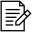
\includegraphics{./img/alg.png}

\begin{verbatim}
const
    MAX_TEMP: integer = 2;
end const

algorithm lecturaTemperatures

    var
        vTemperatures: vector[MAX_TEMP] of float;
    end var

    writeString("Introdueix la lectura 1 : ");
    vTemperatures[1] := readReal();

    writeString("Introdueix la lectura 2 : ");
    vTemperatures[2] := readReal();
    
    writeString("Els valors introduïts han estat : ");
    
    writeString("> Valor de la posició ");
    writeInteger(1);
    writeString(" : ");
    writeReal(vTemperatures[1]);
    
    writeString("> Valor de la posició ");
    writeInteger(2);
    writeString(" : ");
    writeReal(vTemperatures[2]);

end algorithm
\end{verbatim}

I en llenguatge C:


\includegraphics{./img/c.png}

\begin{Shaded}
\begin{Highlighting}[]
\PreprocessorTok{#include }\ImportTok{<stdio.h>}

\PreprocessorTok{#define MAX_TEMP 2}

\DataTypeTok{int}\NormalTok{ main(}\DataTypeTok{int}\NormalTok{ argc, }\DataTypeTok{char}\NormalTok{ **argv) \{}

    \DataTypeTok{float}\NormalTok{ vTemperatures[MAX_TEMP];}
    \DataTypeTok{int}\NormalTok{ i;}

\NormalTok{    printf(}\StringTok{"Introdueix la lectura 1 : "}\NormalTok{);}
\NormalTok{    scanf(}\StringTok{"%f"}\NormalTok{, &vTemperatures[}\DecValTok{0}\NormalTok{]);}

\NormalTok{    printf(}\StringTok{"Introdueix la lectura 2 : "}\NormalTok{);}
\NormalTok{    scanf(}\StringTok{"%f"}\NormalTok{, &vTemperatures[}\DecValTok{1}\NormalTok{]);}
    
\NormalTok{    printf(}\StringTok{"> Valor de la posició %d : %.1f }\SpecialCharTok{\textbackslash{}n}\StringTok{"}\NormalTok{, }\DecValTok{0}\NormalTok{, vTemperatures[}\DecValTok{0}\NormalTok{]);}
\NormalTok{    printf(}\StringTok{"> Valor de la posició %d : %.1f }\SpecialCharTok{\textbackslash{}n}\StringTok{"}\NormalTok{, }\DecValTok{1}\NormalTok{, vTemperatures[}\DecValTok{1}\NormalTok{]);}

    \ControlFlowTok{return} \DecValTok{0}\NormalTok{;}
\NormalTok{\}}
\end{Highlighting}
\end{Shaded}

Cal remarcar una diferència important:

\begin{itemize}
\tightlist
\item
  En \textbf{llenguatge algorísmic} les posicions del vector van des
  \textbf{de la 1 fins a la N}, sent N el número total d'elements del
  vector.
\item
  En \textbf{llenguatge C}, van des \textbf{de la 0 fins a la N-1}, sent
  N el número total d'elements del vector.
\end{itemize}

\section{Stack smashing detected}\label{stack-smashing-detected}

Aquest missatge d'error es produeix quan s'intenta accedir/operar amb
una posició d'un vector que no l'hem definit prèviament. Es pot donar
per diferents situacions que acaben generant el mateix problema.

\begin{itemize}
\tightlist
\item
  Cas 1: es defineix un vector de n-posicions, però en comptes de
  començar per la posició 0 ho fem per la 1. Això és incorrecte:
  recordeu que en C la posició inicial d'un vector sempre és la 0, i la
  final sempre és mida-1. Exemple, per un vector de 3 posicions tindrem:
\end{itemize}

\begin{Shaded}
\begin{Highlighting}[]
\DataTypeTok{int}\NormalTok{ v[}\DecValTok{3}\NormalTok{];}

\NormalTok{v[}\DecValTok{0}\NormalTok{] = }\DecValTok{10}\NormalTok{;  }\CommentTok{/* posició del vector vàlida */}
\NormalTok{v[}\DecValTok{1}\NormalTok{] = }\DecValTok{13}\NormalTok{;  }\CommentTok{/* posició del vector vàlida */}
\NormalTok{v[}\DecValTok{2}\NormalTok{] = }\DecValTok{24}\NormalTok{;  }\CommentTok{/* posició del vector vàlida */}
\NormalTok{v[}\DecValTok{3}\NormalTok{] = }\DecValTok{0}\NormalTok{;   }\CommentTok{/* posició del vector no vàlida! */}
\end{Highlighting}
\end{Shaded}

\begin{itemize}
\tightlist
\item
  Cas 2: es defineix un vector amb menys posicions de les que
  necessitem. Per exemple, si tenim:
\end{itemize}

\begin{Shaded}
\begin{Highlighting}[]
\DataTypeTok{int}\NormalTok{ v[}\DecValTok{2}\NormalTok{];}
\end{Highlighting}
\end{Shaded}

Significa que les posicions reservades en memòria per aquest vector són:

\begin{Shaded}
\begin{Highlighting}[]
\NormalTok{v[}\DecValTok{0}\NormalTok{] = }\DecValTok{10}\NormalTok{;  }\CommentTok{/* posició del vector vàlida */}
\NormalTok{v[}\DecValTok{1}\NormalTok{] = }\DecValTok{13}\NormalTok{;  }\CommentTok{/* posició del vector vàlida */}
\NormalTok{v[}\DecValTok{2}\NormalTok{] = }\DecValTok{24}\NormalTok{;  }\CommentTok{/* posició del vector no vàlida! */}
\end{Highlighting}
\end{Shaded}

Per tant qualsevol operació amb \texttt{v{[}2{]}} ens generarà l'error
indicat. Si volem que el vector contingui 3 elements només cal definir
correctament la seva mida:

\begin{Shaded}
\begin{Highlighting}[]
\DataTypeTok{int}\NormalTok{ v[}\DecValTok{3}\NormalTok{];}
\end{Highlighting}
\end{Shaded}

\chapter{PAC04}\label{pac04}

\section{Com tractar elements d'un vector amb un
bucle}\label{com-tractar-elements-dun-vector-amb-un-bucle}

Imaginem que ens demanen un programa que realitzi dues accions:

\begin{enumerate}
\def\labelenumi{\arabic{enumi}.}
\tightlist
\item
  llegir des del canal estàndard d'entrada (teclat) 5 números i
  introduir-los en un vector d'enters.
\item
  mostrar pel canal estàndard de sortida (pantalla) els 5 números del
  vector d'enters del punt anterior.
\end{enumerate}

L'algorisme podria ser el següent:

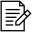
\includegraphics{./img/alg.png}

\begin{verbatim}
const
   MAX_NUMS: integer = 5;
end const

algorithm vectorDeNumeros

   var
      i: integer;
      vectorNumeros: vector[MAX_NUMS] of integer;
   end var

   { Assignar valor a cada posició del vector des de teclat }
   for i := 1 to MAX_NUMS do
      writeString("Introdueix número : ");
      vectorNumeros[i] := readInteger();
   end for

   { Mostrar per pantalla quin valor hi ha a cada posició del vector:}
   { es podria haver utilitzat un bucle for, però ho implemento amb un while }
   { perquè es vegi que també és possible fer-ho }
   i := 1;

   while i ≤ MAX_NUMS do

      writeString("La posició ");
      writeInteger(i);
      writeString(" del vector conté el número ");
      writeInteger(vectorNumeros[i]);

      { És molt important que amb un bucle while incrementem la variable que utilitzem d'índex }
      { abans de finalitzar tot el bloc d'instruccions que executa, ja que en cas contrari el seu }
      { valor sempre seria de i == 1 }
      i := i+1;

   end while

end algorithm
\end{verbatim}

Com es pot veure, per tal d'insertar/llegir els elements d'un vector
aprofitem la iteració d'un bucle per recorre'ls tots, un a un,
mitjançant una variable que utilitzem d'índex (en aquests casos, la
variable \texttt{i}).

La traducció a C de l'algorisme podria ser així:


\includegraphics{./img/c.png}

\begin{Shaded}
\begin{Highlighting}[]
\PreprocessorTok{#include }\ImportTok{<stdio.h>}

\PreprocessorTok{#define MAX_NUMS 5}

\DataTypeTok{int}\NormalTok{ main(}\DataTypeTok{int}\NormalTok{ argc, }\DataTypeTok{char}\NormalTok{ **argv) \{}

   \DataTypeTok{int}\NormalTok{ vectorNumeros [MAX_NUMS];}
   \DataTypeTok{int}\NormalTok{ i;}

   \CommentTok{/* Assignar valor a cada posició del vector des de teclat */}
   \ControlFlowTok{for}\NormalTok{ (i = }\DecValTok{0}\NormalTok{; i < MAX_NUMS; i++) \{}
\NormalTok{      printf(}\StringTok{"Introdueix número : "}\NormalTok{);}
\NormalTok{      scanf(}\StringTok{"%d"}\NormalTok{, &vectorNumeros[i]);}
\NormalTok{   \}}

   \CommentTok{/* Mostrar per pantalla quin valor hi ha a cada posició del vector:}
\CommentTok{      es podria haver utilitzat un bucle for, però ho implemento amb un while}
\CommentTok{      perquè es vegi que també és possible fer-ho */}
\NormalTok{   i = }\DecValTok{0}\NormalTok{;}

   \ControlFlowTok{while}\NormalTok{ (i < MAX_NUMS) \{}

\NormalTok{      printf(}\StringTok{"}\SpecialCharTok{\textbackslash{}n}\StringTok{La posició %d del vector conté el número %d"}\NormalTok{, i, vectorNumeros[i]);}

      \CommentTok{/* És molt important que amb un bucle while incrementem la variable que utilitzem d'índex}
\CommentTok{         abans de finalitzar tot el bloc d'instruccions que executa, ja que en cas contrari el seu}
\CommentTok{         valor sempre seria de i == 0 */}
\NormalTok{      i = i+}\DecValTok{1}\NormalTok{;}
\NormalTok{   \}}
\NormalTok{\}}
\end{Highlighting}
\end{Shaded}

\section{Entrada continua de valors amb un
bucle}\label{entrada-continua-de-valors-amb-un-bucle}

Imaginem que hem de fer un programa que vagi demanant números
indefinidament i que finalitzi únicament en el cas que el número
introduit sigui parell.

Una possible forma de fer-ho utilitzant un únic while seria la següent:


\includegraphics{./img/c.png}

\begin{Shaded}
\begin{Highlighting}[]
\PreprocessorTok{#include }\ImportTok{<stdio.h>}

\DataTypeTok{int}\NormalTok{ main(}\DataTypeTok{int}\NormalTok{ argc, }\DataTypeTok{char}\NormalTok{ **argv) \{}

   \DataTypeTok{int}\NormalTok{ numero;}

   \CommentTok{/* Demanem una primera vegada el número a validar}
\CommentTok{      just abans d'entrar al bucle */}
\NormalTok{   printf(}\StringTok{"Tecleja un número parell : "}\NormalTok{);}
\NormalTok{   scanf(}\StringTok{"%d"}\NormalTok{, &numero);}

   \ControlFlowTok{while}\NormalTok{ ((numero % }\DecValTok{2}\NormalTok{) != }\DecValTok{0}\NormalTok{) \{}

      \CommentTok{/* Entra al bucle en el cas que el}
\CommentTok{         residu de la divisió per 2 sigui }
\CommentTok{         diferent de 0 (equival a no ser parell) */}
\NormalTok{      printf(}\StringTok{"El número %d no és parell !!}\SpecialCharTok{\textbackslash{}n}\StringTok{"}\NormalTok{, numero);}

      \CommentTok{/* Tornem a demanar un número, ara ja}
\CommentTok{         dins del bucle */}
\NormalTok{      printf(}\StringTok{"Tecleja un número parell : "}\NormalTok{);}
\NormalTok{      scanf(}\StringTok{"%d"}\NormalTok{, &numero);}
\NormalTok{   \}}

\NormalTok{   printf(}\StringTok{"El número %d és parell.}\SpecialCharTok{\textbackslash{}n}\StringTok{"}\NormalTok{, numero);}
   \ControlFlowTok{return} \DecValTok{0}\NormalTok{;}
\NormalTok{\}}
\end{Highlighting}
\end{Shaded}

Abans d'entrar al bucle demanem un el valor de la variable numero. A
continuació s'utilitza la condició de bucle per validar si es tracta
d'un número parell o senar:

\begin{itemize}
\tightlist
\item
  Si el número es parell, no s'entra al bucle.
\item
  Si el número és senar es compleix la condició del bucle i s'hi entra;
  dins del bucle es torna a demanar un valor per la variable numero i es
  torna a actuar igual que abans:

  \begin{itemize}
  \tightlist
  \item
    Si és senar, no se surt del bucle.
  \item
    En cas contrari, se surt del bucle.
  \end{itemize}
\end{itemize}

Finalment es mostra per pantalla el missatge ``El número X és parell''.

\chapter{PAC05}\label{pac05}

\section{Exemple: nomines}\label{exemple-nomines}

Imaginem que volem un programa que ens permeti entrar les nòmines de
tots els empleats de la nostra empresa. Un empleat el definim com a nom
(cadena de caràcters) + nòmina (real). El programa ha de mostrar al
final de tot la relació de nòmines de tots els empleats, la mitjana de
totes les nòmines de l'empresa, i qui cobra més i menys a l'empresa.

Una possible forma de programa-ho seria la següent:


\includegraphics{./img/c.png}

\begin{Shaded}
\begin{Highlighting}[]
\PreprocessorTok{#include }\ImportTok{<stdio.h>}
\PreprocessorTok{#include }\ImportTok{<string.h>}

\PreprocessorTok{#define MAX_EMPLEATS 5}
\PreprocessorTok{#define MAX_NOM 20+1}

\KeywordTok{typedef} \KeywordTok{struct}\NormalTok{ \{}
   \DataTypeTok{char}\NormalTok{ nom[MAX_NOM];}
   \DataTypeTok{float}\NormalTok{ nomina;}
\NormalTok{\} tEmpleat;}

\DataTypeTok{int}\NormalTok{ main(}\DataTypeTok{int}\NormalTok{ argc, }\DataTypeTok{char}\NormalTok{ **argv) \{}

\NormalTok{   tEmpleat vEmpleats[MAX_EMPLEATS];}
   \DataTypeTok{int}\NormalTok{ i = }\DecValTok{0}\NormalTok{;}
   \DataTypeTok{int}\NormalTok{ maxNomina = }\DecValTok{0}\NormalTok{;}
   \DataTypeTok{int}\NormalTok{ minNomina = }\DecValTok{0}\NormalTok{;}
   \DataTypeTok{float}\NormalTok{ sumaNomines = }\DecValTok{0}\NormalTok{;}

   \ControlFlowTok{for}\NormalTok{ (i=}\DecValTok{0}\NormalTok{; i<MAX_EMPLEATS; i++) \{}
\NormalTok{      printf(}\StringTok{"}\SpecialCharTok{\textbackslash{}n}\StringTok{Nom empleat : "}\NormalTok{);}
\NormalTok{      scanf(}\StringTok{"%s"}\NormalTok{, vEmpleats[i].nom);}
\NormalTok{      printf(}\StringTok{"Nòmina : "}\NormalTok{);}
\NormalTok{      scanf(}\StringTok{"%f"}\NormalTok{, &vEmpleats[i].nomina);}
\NormalTok{   \}}

\NormalTok{   printf(}\StringTok{"}\SpecialCharTok{\textbackslash{}n}\StringTok{Llistat de nòmines d'empleats : }\SpecialCharTok{\textbackslash{}n\textbackslash{}n}\StringTok{"}\NormalTok{);}

   \ControlFlowTok{for}\NormalTok{ (i=}\DecValTok{0}\NormalTok{; i<MAX_EMPLEATS; i++) \{}
\NormalTok{      sumaNomines = sumaNomines + vEmpleats[i].nomina;}
      \ControlFlowTok{if}\NormalTok{ (vEmpleats[i].nomina > vEmpleats[maxNomina].nomina) \{}
\NormalTok{         maxNomina = i;}
\NormalTok{      \}}
      \ControlFlowTok{if}\NormalTok{ (vEmpleats[i].nomina < vEmpleats[minNomina].nomina) \{}
\NormalTok{         minNomina = i;}
\NormalTok{      \}}
\NormalTok{      printf(}\StringTok{"%s --> %.2f €}\SpecialCharTok{\textbackslash{}n}\StringTok{"}\NormalTok{, vEmpleats[i].nom, vEmpleats[i].nomina);}
\NormalTok{   \}}

\NormalTok{   printf(}\StringTok{"}\SpecialCharTok{\textbackslash{}n}\StringTok{Mitjana nònimes : %.2f €"}\NormalTok{, sumaNomines/MAX_EMPLEATS);}
\NormalTok{   printf(}\StringTok{"}\SpecialCharTok{\textbackslash{}n}\StringTok{Nòmina més alta : %.2f € (%s)"}\NormalTok{, vEmpleats[maxNomina].nomina, vEmpleats[maxNomina].nom);}
\NormalTok{   printf(}\StringTok{"}\SpecialCharTok{\textbackslash{}n}\StringTok{Nòmina més baixa : %.2f € (%s)"}\NormalTok{, vEmpleats[minNomina].nomina, vEmpleats[minNomina].nom);}
\NormalTok{\}}
\end{Highlighting}
\end{Shaded}

Com es pot veure, s'utilitza un vector de \texttt{tEmpleat} de forma que
donada una longitud màxima del vector, anirem introduint els tEmpleats
un a un dins d'ell. Una vegada fet, ja podem tornar a recórrer el vector
de tEmpleat i realitzar tots els càlculs que ens demanen, així com
mostrar per pantalla les nòmines de tots els empleats.

En aquest exemple la variable i fa d'índex per recórrer el vector, i les
variables maxNomina i minNomina també són índexos: indiquen en quina
posició estàn els empleats amb la nòmina més alta i més baixa
respectivament.

\section{Exemple accions}\label{exemple-accions}

Adjunto un exemple inventat de com es poden definir accions que permetin
modificar els atributs d'una tupla passada com a punter.


\includegraphics{./img/c.png}

\begin{Shaded}
\begin{Highlighting}[]
\PreprocessorTok{#include }\ImportTok{<stdio.h>}

\PreprocessorTok{#define MAX_CHAR 10+1}

\KeywordTok{typedef} \KeywordTok{struct}\NormalTok{ \{}
   \DataTypeTok{char}\NormalTok{ nom[MAX_CHAR];}
   \DataTypeTok{float}\NormalTok{ nomina;}
\NormalTok{\} tEmpleat;}

\CommentTok{/* Predeclaració de les accions */}

\DataTypeTok{void}\NormalTok{ printEmpleat(tEmpleat empleat);}
\DataTypeTok{void}\NormalTok{ setNominaEmpleat(tEmpleat *empleat, }\DataTypeTok{float}\NormalTok{ nomina);}
\DataTypeTok{void}\NormalTok{ setNomEmpleat(tEmpleat *empleat, }\DataTypeTok{char}\NormalTok{ nom[MAX_CHAR]);}

\DataTypeTok{int}\NormalTok{ main(}\DataTypeTok{int}\NormalTok{ argc, }\DataTypeTok{char}\NormalTok{* argv[]) \{}

   \CommentTok{/* Declarem nouEmpleat de tipus tEmpleat,}
\CommentTok{      però no li donarem cap valor directament}
\CommentTok{      als seus dos atributs (nom i nomina): ho }
\CommentTok{      farem mitjançant dues accions */}
\NormalTok{   tEmpleat nouEmpleat;}
   
   \CommentTok{/* Els valors dels atributs nom i nomina els}
\CommentTok{      llegirem des de teclat i els desarem inicialment}
\CommentTok{      en les següents dues variables */}
   \DataTypeTok{char}\NormalTok{ nom[MAX_CHAR];}
   \DataTypeTok{float}\NormalTok{ nomina;}
   
\NormalTok{   printf(}\StringTok{"}\SpecialCharTok{\textbackslash{}n}\StringTok{Nom empleat : "}\NormalTok{);}
\NormalTok{   scanf(}\StringTok{"%s"}\NormalTok{, nom);}
      
\NormalTok{   printf(}\StringTok{"Nòmina empleat : "}\NormalTok{);}
\NormalTok{   scanf(}\StringTok{"%f"}\NormalTok{, &nomina);}
   
   \CommentTok{/* Assignem el nom i la nòmina al tEmpleat empleat1}
\CommentTok{      utilitzant les accions definides. Fixeu-vos}
\CommentTok{      que el paràmetre nouEmpleat el passem com a punter}
\CommentTok{      (passem la seva adreça en memòria, ja que va }
\CommentTok{      precedit per &) */}
\NormalTok{   setNomEmpleat(&nouEmpleat, nom);}
\NormalTok{   setNominaEmpleat(&nouEmpleat, nomina);}
   
   \CommentTok{/* Mostrem les dades de la tupla tEmpleat empleat1}
\CommentTok{      per pantalla */}
\NormalTok{   printEmpleat(nouEmpleat);}

   \ControlFlowTok{return} \DecValTok{0}\NormalTok{;}
\NormalTok{\}}

\CommentTok{/* Implementació de les accions */}

\DataTypeTok{void}\NormalTok{ printEmpleat(tEmpleat empleat) \{}
    
   \CommentTok{/* El paràmetre empleat és d'entrada, amb el}
\CommentTok{      que l'accés als seus atributs ho farem}
\CommentTok{      amb un punt : empleat.nom, empleat.nomina */}
\NormalTok{   printf(}\StringTok{"}\SpecialCharTok{\textbackslash{}n}\StringTok{Dades de l'empleat: }\SpecialCharTok{\textbackslash{}n}\StringTok{"}\NormalTok{);}
\NormalTok{   printf(}\StringTok{"}\SpecialCharTok{\textbackslash{}t}\StringTok{Nom: %s}\SpecialCharTok{\textbackslash{}n}\StringTok{"}\NormalTok{, empleat.nom);}
\NormalTok{   printf(}\StringTok{"}\SpecialCharTok{\textbackslash{}t}\StringTok{Nòmina: %.2f €}\SpecialCharTok{\textbackslash{}n}\StringTok{"}\NormalTok{, empleat.nomina);}
\NormalTok{\}}

\DataTypeTok{void}\NormalTok{ setNominaEmpleat(tEmpleat *empleat, }\DataTypeTok{float}\NormalTok{ nomina) \{}
    
   \CommentTok{/* El paràmetre empleat (de tipus inout) és un punter,}
\CommentTok{      per tal que des de dins de l'acció sigui possible}
\CommentTok{      modificar el valor (d'un atribut) de l'empleat}
\CommentTok{      definit al main del nostre programa.}
\CommentTok{      L'accés a un atribut d'un element referenciat amb}
\CommentTok{      un punter es fa amb '->' : empleat->nomina. */}
\NormalTok{    empleat->nomina = nomina;}
\NormalTok{\}}

\DataTypeTok{void}\NormalTok{ setNomEmpleat(tEmpleat *empleat, }\DataTypeTok{char}\NormalTok{ nom[MAX_CHAR]) \{}
    
   \CommentTok{/* Idem que en l'acció setNominaEmpleat. En aquest cas}
\CommentTok{      a més a més cal recordar que l'assignació d'strings}
\CommentTok{      la fem amb la funció strcpy de C, en comptes }
\CommentTok{      d'utilitzar l'assignació habitual dels tipus }
\CommentTok{      primitius (char, int, float, ...) */}
\NormalTok{   strcpy(empleat->nom, nom);}
\NormalTok{\}}
\end{Highlighting}
\end{Shaded}

\section{Comanda scanf}\label{comanda-scanf}

Quan utilitzem la comanda \texttt{scanf} fins ara sempre li hem passat
el nom de la variable precedit per\texttt{\&}. Això significa que
realment a aquesta comanda li estem passant la posició de la memòria on
resideix la variable que li indiquem.

Així, per exemple, quan fem la següent operació
\texttt{scanf("\%d",\ \&numero);} estem passant el valor que introduïm
per teclat directament a la posició de memòria on tenim desada la
variable numero. D'aquí ve utilitzar \texttt{\&numero} en comptes de
\texttt{numero}. El mateix comportament tenim pels tipus primitius
\texttt{char}, \texttt{float}, etc.

Els vectors de caràcters en llenguatge C tenen una característica: el
nom de l'array conté l'adreça de memòria on està desada la primera
posició de l'array.

Per exemple, quan executem \texttt{scanf("\%s",\ cadena);} el valor de
cadena és l'adreça de memòria inicial on està ubicat l'array. Dit d'una
altra manera, cadena conté el mateix valor que \texttt{\&cadena{[}0{]}}
(és una altra forma que tenim per referir-nos a la posició inicial en
memòria de l'array).

Adjunto un exemple amb tots aquests conceptes:


\includegraphics{./img/c.png}

\begin{Shaded}
\begin{Highlighting}[]
\PreprocessorTok{#include }\ImportTok{<stdio.h>}
\PreprocessorTok{#define MAXIM 10}

\DataTypeTok{int}\NormalTok{ main(}\DataTypeTok{int}\NormalTok{ argc, }\DataTypeTok{char}\NormalTok{ **argv) \{}

    \DataTypeTok{char}\NormalTok{ cadena[MAXIM];}
    \DataTypeTok{int}\NormalTok{ numero;}

\NormalTok{    printf(}\StringTok{"Reservada la posició de memòria %p per la variable numero}\SpecialCharTok{\textbackslash{}n}\StringTok{"}\NormalTok{, &numero);}
\NormalTok{    printf(}\StringTok{"Reservada la posició de memòria %p per la variable cadena}\SpecialCharTok{\textbackslash{}n}\StringTok{"}\NormalTok{, cadena);}
\NormalTok{    printf(}\StringTok{"Reservada la posició de memòria %p per la variable cadena}\SpecialCharTok{\textbackslash{}n}\StringTok{"}\NormalTok{, &cadena[}\DecValTok{0}\NormalTok{]);}

\NormalTok{    printf(}\StringTok{"}\SpecialCharTok{\textbackslash{}n}\StringTok{Introdueix un número enter: "}\NormalTok{);}
\NormalTok{    scanf(}\StringTok{"%d"}\NormalTok{, &numero);}
\NormalTok{    printf(}\StringTok{"}\SpecialCharTok{\textbackslash{}n}\StringTok{Introdueix una cadena: "}\NormalTok{);}
\NormalTok{    scanf(}\StringTok{"%s"}\NormalTok{,cadena);}

\NormalTok{    printf(}\StringTok{"}\SpecialCharTok{\textbackslash{}n}\StringTok{Has assignat els següents valors :}\SpecialCharTok{\textbackslash{}n}\StringTok{"}\NormalTok{);}
\NormalTok{    printf(}\StringTok{"numero = %d }\SpecialCharTok{\textbackslash{}n}\StringTok{"}\NormalTok{, numero);}
\NormalTok{    printf(}\StringTok{"cadena = %s }\SpecialCharTok{\textbackslash{}n}\StringTok{"}\NormalTok{, cadena);}

    \ControlFlowTok{return} \DecValTok{0}\NormalTok{;}
\NormalTok{\}}
\end{Highlighting}
\end{Shaded}

\section{\texorpdfstring{Finalitzador
`\textbackslash{}0'}{Finalitzador \textbackslash{}0}}\label{finalitzador-0}

Com es va veure al mòdul \textbf{Cadenes de caràcters en C} de la xWiki,
\emph{``una cadena de caràcters o string és una seqüència de caràcters
finalitzada pel caràcter `\textbackslash{}0'\,''}. Per tant hem de tenir
en compte que el finalitzador `\textbackslash{}0' càpiga a la nostra
variable, ja que aquesta és la forma que té C de saber on s'acaba un
string en memòria.

Imaginem que tenim tres cadenes, amb el mateix contingut però de mida
diferent (podem tenir posicions buides). Què passa si les comparem? I si
comparem amb una cadena de mateix contingut però sense finalitzador
`\textbackslash{}0'?


\includegraphics{./img/c.png}

\begin{Shaded}
\begin{Highlighting}[]
\PreprocessorTok{#include }\ImportTok{<stdio.h>}
\PreprocessorTok{#include }\ImportTok{<string.h>}

\DataTypeTok{int}\NormalTok{ main() \{}

    \DataTypeTok{char}\NormalTok{ ciutat1[}\DecValTok{7}\NormalTok{] = }\StringTok{"Girona"}\NormalTok{;}
    \DataTypeTok{char}\NormalTok{ ciutat2[}\DecValTok{8}\NormalTok{] = }\StringTok{"Girona"}\NormalTok{;}
    \DataTypeTok{char}\NormalTok{ ciutat3[}\DecValTok{6}\NormalTok{] = }\StringTok{"Girona"}\NormalTok{; }\CommentTok{/* no conté el '\textbackslash{}0' final */}

    \CommentTok{/* si strcmp retorna 0 significa que les dues cadenes són iguals */}
\NormalTok{    printf (}\StringTok{"Les variables ciutat1 i ciutat2 són iguals? %d}\SpecialCharTok{\textbackslash{}n}\StringTok{"}\NormalTok{, strcmp(ciutat1, ciutat2));}
\NormalTok{    printf (}\StringTok{"Les variables ciutat1 i ciutat3 són iguals? %d}\SpecialCharTok{\textbackslash{}n}\StringTok{"}\NormalTok{, strcmp(ciutat1, ciutat3));}
\NormalTok{\}}
\end{Highlighting}
\end{Shaded}

La forma que tenim per forçar que una cadena no contingui el
finalitzador és limitant la seva mida als caràcters que contindrà, sense
tenir en compte reservar-ne un pel `\textbackslash{}0'. En aquest cas ho
fem amb char \texttt{ciutat3{[}6{]}\ =\ "Girona"}.

La sortida generada és la següent:

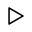
\includegraphics{./img/play.png}

\begin{Shaded}
\begin{Highlighting}[]
\NormalTok{Les variables ciutat1 i ciutat2 són iguals? }\DecValTok{0}
\NormalTok{Les variables ciutat1 i ciutat3 són iguals? -}\DecValTok{1}
\end{Highlighting}
\end{Shaded}

D'aquí la importància del finalitzador de cadenes de caràcters. Per
tant, si per exemple ens diuen que tindrem una variable x de tipus
string i de mida màxima 15, realment al nostre programa la definirem amb
longitud 15+1, per tal que hi càpiga el finalitzador `\textbackslash{}0'
en cas que s'ocupin els 15 caràcters anteriors.

\chapter{PAC06}\label{pac06}

\section{Comanda strcmp}\label{comanda-strcmp}

La funció \texttt{strcmp} de C fa una comparació caràcter a caràcter de
dos cadenes i com a resultat:

\begin{itemize}
\tightlist
\item
  Retorna 0: si les dues cadenes són iguals
\item
  Retorna -1: si la primera cadena \textless{} segona cadena
\item
  Retorna 1: si la primera cadena \textgreater{} segona cadena
\end{itemize}

Com funciona una comparació caràcter a caràcter? Imaginem que tenim els
següents dos string: ``UOC'' i ``UAB''.

La comparació caràcter a caràcter que realitza la funció strcmp és la
següent:

\begin{itemize}
\tightlist
\item
  Caràcters de la posició 0 dels dos string: \textbf{U}OC vs
  \textbf{U}AB. Són iguals, amb el que passa a comparar el següent
  caràcter.
\item
  Caràcters de la posició 1 dels dos string: U\textbf{O}C vs
  U\textbf{A}B. Són diferents (`O' \textgreater{} `A'), finalitza la
  comparació i la funció \texttt{strcmp} retorna el valor 1.
\end{itemize}

Per si vols fer proves, aquest exemple codificat en C podria ser:


\includegraphics{./img/c.png}

\begin{Shaded}
\begin{Highlighting}[]
\PreprocessorTok{#include }\ImportTok{<stdio.h>}
\PreprocessorTok{#include }\ImportTok{<string.h>}

\PreprocessorTok{#define MAX_STRING 3+1}

\DataTypeTok{int}\NormalTok{ main(}\DataTypeTok{int}\NormalTok{ argc, }\DataTypeTok{char}\NormalTok{ **argv) \{}

    \DataTypeTok{char}\NormalTok{ cadena1[MAX_STRING] = }\StringTok{"UOC"}\NormalTok{;}
    \DataTypeTok{char}\NormalTok{ cadena2[MAX_STRING] = }\StringTok{"UAB"}\NormalTok{;}
    \DataTypeTok{int}\NormalTok{ resultatComparacio = }\DecValTok{0}\NormalTok{;}

\NormalTok{    resultatComparacio = strcmp(cadena1, cadena2);}

\NormalTok{    printf(}\StringTok{"Comparació strings }\SpecialCharTok{\textbackslash{}"}\StringTok{%s}\SpecialCharTok{\textbackslash{}"}\StringTok{ i }\SpecialCharTok{\textbackslash{}"}\StringTok{%s}\SpecialCharTok{\textbackslash{}"}\StringTok{ = %d}\SpecialCharTok{\textbackslash{}n}\StringTok{"}\NormalTok{, cadena1, cadena2, resultatComparacio);}

    \ControlFlowTok{if}\NormalTok{ (resultatComparacio == }\DecValTok{0}\NormalTok{) \{}
\NormalTok{        printf(}\StringTok{"El resultat %d significa que l'string }\SpecialCharTok{\textbackslash{}"}\StringTok{%s}\SpecialCharTok{\textbackslash{}"}\StringTok{ == string }\SpecialCharTok{\textbackslash{}"}\StringTok{%s}\SpecialCharTok{\textbackslash{}"\textbackslash{}n}\StringTok{"}\NormalTok{, resultatComparacio, cadena1, cadena2);}
\NormalTok{    \} }\ControlFlowTok{else} \ControlFlowTok{if}\NormalTok{ (resultatComparacio == -}\DecValTok{1}\NormalTok{) \{}
\NormalTok{        printf(}\StringTok{"El resultat %d significa que l'string }\SpecialCharTok{\textbackslash{}"}\StringTok{%s}\SpecialCharTok{\textbackslash{}"}\StringTok{ < string }\SpecialCharTok{\textbackslash{}"}\StringTok{%s}\SpecialCharTok{\textbackslash{}"\textbackslash{}n}\StringTok{"}\NormalTok{, resultatComparacio, cadena1, cadena2);}
\NormalTok{    \} }\ControlFlowTok{else} \ControlFlowTok{if}\NormalTok{ (resultatComparacio == }\DecValTok{1}\NormalTok{) \{}
\NormalTok{        printf(}\StringTok{"El resultat %d significa que l'string }\SpecialCharTok{\textbackslash{}"}\StringTok{%s}\SpecialCharTok{\textbackslash{}"}\StringTok{ > string }\SpecialCharTok{\textbackslash{}"}\StringTok{%s}\SpecialCharTok{\textbackslash{}"\textbackslash{}n}\StringTok{"}\NormalTok{, resultatComparacio, cadena1, cadena2); }
\NormalTok{    \}}

    \ControlFlowTok{return} \DecValTok{0}\NormalTok{;}
\NormalTok{\}}
\end{Highlighting}
\end{Shaded}

En què es basa strcmp per decidir que `O' \textgreater{} `A' ? en el
valor ASCII (numèric) que té associat cada caràcter. Per aquest motiu és
normal que interpreti diferent una `A' i una `a', ja que són caràcters
diferents; de fet segons els valors ASCII, tenim que `A' \textless{}
`a'.

Per si no vols consultar la taula ASCII per internet, pots obtenir tu
mateix els valors de cada caràcter de la següent forma:


\includegraphics{./img/c.png}

\begin{Shaded}
\begin{Highlighting}[]
\PreprocessorTok{#include }\ImportTok{<stdio.h>}

\DataTypeTok{int}\NormalTok{ main(}\DataTypeTok{int}\NormalTok{ argc, }\DataTypeTok{char}\NormalTok{ **argv) \{}

    \DataTypeTok{int}\NormalTok{ i = }\DecValTok{0}\NormalTok{;}

    \CommentTok{/* Relació de caràcters ASCII (només és un subconjunt!)}
\CommentTok{       ordenats de més petit a més gran */}
    \ControlFlowTok{for}\NormalTok{ (i=}\DecValTok{33}\NormalTok{; i<=}\DecValTok{126}\NormalTok{; i++) \{}
\NormalTok{        printf(}\StringTok{"%d : %c}\SpecialCharTok{\textbackslash{}n}\StringTok{"}\NormalTok{, i, i);}
\NormalTok{    \}}
\NormalTok{\}}
\end{Highlighting}
\end{Shaded}

\section{Exemple}\label{exemple}

Imaginem que treballem amb els empleats d'una empresa. Posem per cas que
després d'introduir n-empleats al nostre sistema, volem una funció que
ens retorni l'empleat que té la nòmina més petita.

Com que esperem un valor de retorn, estem davant d'una funció. A la
funció li passarem un vector d'empleats amb tots els empleats que
prèviament hem introduit a la nostra empresa.

Sense entrar en la codificació de la funció, el main del nostre programa
pot ser similar al següent:

\includegraphics{./img/c.png}

\begin{Shaded}
\begin{Highlighting}[]
\PreprocessorTok{#include }\ImportTok{<stdio.h>}
\PreprocessorTok{#include }\ImportTok{<string.h>}

\PreprocessorTok{#define MAX_EMPLEATS 2}
\PreprocessorTok{#define MAX_CARACTERS 20+1}

\KeywordTok{typedef} \KeywordTok{struct}\NormalTok{ \{}
    \DataTypeTok{char}\NormalTok{ nom[MAX_CARACTERS];}
    \DataTypeTok{char}\NormalTok{ cognom[MAX_CARACTERS];}
    \DataTypeTok{float}\NormalTok{ nomina;}
\NormalTok{\} tEmpleat;}

\DataTypeTok{int}\NormalTok{ main(}\DataTypeTok{int}\NormalTok{ argc, }\DataTypeTok{char}\NormalTok{ **argv) \{}

\NormalTok{    tEmpleat vEmpleats[MAX_EMPLEATS];}
    \DataTypeTok{int}\NormalTok{ i = }\DecValTok{0}\NormalTok{;}

    \ControlFlowTok{for}\NormalTok{ (i=}\DecValTok{0}\NormalTok{; i<MAX_EMPLEATS; i++) \{}

\NormalTok{        printf(}\StringTok{"}\SpecialCharTok{\textbackslash{}n}\StringTok{Nom empleat %d : "}\NormalTok{, i);}
\NormalTok{        scanf(}\StringTok{"%s"}\NormalTok{, vEmpleats[i].nom);}

\NormalTok{        printf(}\StringTok{"Cognom empleat %d : "}\NormalTok{, i);}
\NormalTok{        scanf(}\StringTok{"%s"}\NormalTok{, vEmpleats[i].cognom);}

\NormalTok{        printf(}\StringTok{"Nòmina empleat %d : "}\NormalTok{, i);}
\NormalTok{        scanf(}\StringTok{"%f"}\NormalTok{, &vEmpleats[i].nomina);}

\NormalTok{    \}}

\NormalTok{    tEmpleat empleat = cercaEmpleatNominaMinima(vEmpleats);}
\NormalTok{    printf(}\StringTok{"}\SpecialCharTok{\textbackslash{}n}\StringTok{L'empleat amb la nòmina més baixa és %s, %s (%.2f €)"}\NormalTok{, empleat.cognom, empleat.nom, empleat.nomina);}
    \ControlFlowTok{return} \DecValTok{0}\NormalTok{;}
\NormalTok{\}}
\end{Highlighting}
\end{Shaded}

Fins aquest punt no hi ha res nou: utilitzem en aquest cas un vector de
\texttt{tEmpleat} per tal d'anar introduint els empleats per teclat, i
per cada empleat demanem el nom, el cognom i la seva nòmina.

El que cal fer ara és implementar la funció
\texttt{cercaEmpleatNominaMinima}, que rep com a paràmetre el vector
d'empleats de l'empresa.

De moment oblidem-nos que estem davant d'una funció, simplement
centrem-nos en quina és l'acció que volem fer. En aquest cas, volem fer
un programa que recorri un a un tots els elements d'un vector, i trobi
l'empleat que cobra menys.

Una possible codificació seria la següent:

\includegraphics{./img/c.png}

\begin{Shaded}
\begin{Highlighting}[]
\DataTypeTok{int}\NormalTok{ i = }\DecValTok{0}\NormalTok{; }
\DataTypeTok{int}\NormalTok{ minNomina = }\DecValTok{0}\NormalTok{;}

\ControlFlowTok{for}\NormalTok{ (i=}\DecValTok{0}\NormalTok{; i<MAX_EMPLEATS; i++) \{}
    \ControlFlowTok{if}\NormalTok{ (vector[i].nomina < vector[minNomina].nomina) \{}
\NormalTok{        minNomina = i;}
\NormalTok{    \}}
\NormalTok{\}}
\end{Highlighting}
\end{Shaded}

Aquest fragment de codi simplement recorre un a un tots els
\texttt{tEmpleat} d'un vector, comparant la nòmina més baixa trobada
fins el moment amb la de l'empleat que està tractant en qüestió, i si
aquesta segona és més baixa, ens quedem amb la seva posició dins del
vector com a empleat amb la nòmina més baixa (és el mateix plantejament
que l'exposat a l'exemple de la setmana passada, per tant fins aquí res
nou).

Ara convertim aquest fragment de codi en una funció:

\includegraphics{./img/c.png}

\begin{Shaded}
\begin{Highlighting}[]
\NormalTok{tEmpleat cercaEmpleatNominaMinima(tEmpleat vector[MAX_EMPLEATS]) \{}

    \DataTypeTok{int}\NormalTok{ i = }\DecValTok{0}\NormalTok{; }
    \DataTypeTok{int}\NormalTok{ minNomina = }\DecValTok{0}\NormalTok{;}

    \ControlFlowTok{for}\NormalTok{ (i=}\DecValTok{0}\NormalTok{; i<MAX_EMPLEATS; i++) \{}
        \ControlFlowTok{if}\NormalTok{ (vector[i].nomina < vector[minNomina].nomina) \{}
\NormalTok{            minNomina = i;}
\NormalTok{        \}}
\NormalTok{    \}}

    \ControlFlowTok{return}\NormalTok{ vector[minNomina];}
\NormalTok{\}}
\end{Highlighting}
\end{Shaded}

Com pots veure l'única diferència és que ara el codi té la capçalera de
la funció, la qual ens diu que rep com a paràmetre un element de tipus
vector de \texttt{tEmpleat}, i que retornarà un element de tipus
\texttt{tEmpleat}.

D'aquesta forma el programa complet queda de la següent manera:

\includegraphics{./img/c.png}

\begin{Shaded}
\begin{Highlighting}[]
\PreprocessorTok{#include }\ImportTok{<stdio.h>}
\PreprocessorTok{#include }\ImportTok{<string.h>}

\PreprocessorTok{#define MAX_EMPLEATS 2}
\PreprocessorTok{#define MAX_CARACTERS 20+1}

\KeywordTok{typedef} \KeywordTok{struct}\NormalTok{ \{}
    \DataTypeTok{char}\NormalTok{ nom[MAX_CARACTERS];}
    \DataTypeTok{char}\NormalTok{ cognom[MAX_CARACTERS];}
    \DataTypeTok{float}\NormalTok{ nomina;}
\NormalTok{\} tEmpleat;}

\CommentTok{/* Predeclaració de funcions/accions */}
\NormalTok{tEmpleat cercaEmpleatNominaMinima(tEmpleat vector[MAX_EMPLEATS]);}

\DataTypeTok{int}\NormalTok{ main(}\DataTypeTok{int}\NormalTok{ argc, }\DataTypeTok{char}\NormalTok{ **argv) \{}

\NormalTok{    tEmpleat vEmpleats[MAX_EMPLEATS];}
    \DataTypeTok{int}\NormalTok{ i = }\DecValTok{0}\NormalTok{;}

    \ControlFlowTok{for}\NormalTok{ (i=}\DecValTok{0}\NormalTok{; i<MAX_EMPLEATS; i++) \{}

\NormalTok{        printf(}\StringTok{"}\SpecialCharTok{\textbackslash{}n}\StringTok{Nom empleat %d : "}\NormalTok{, i);}
\NormalTok{        scanf(}\StringTok{"%s"}\NormalTok{, vEmpleats[i].nom);}

\NormalTok{        printf(}\StringTok{"Cognom empleat %d : "}\NormalTok{, i);}
\NormalTok{        scanf(}\StringTok{"%s"}\NormalTok{, vEmpleats[i].cognom);}

\NormalTok{        printf(}\StringTok{"Nòmina empleat %d : "}\NormalTok{, i);}
\NormalTok{        scanf(}\StringTok{"%f"}\NormalTok{, &vEmpleats[i].nomina);}

\NormalTok{    \}}

\NormalTok{    tEmpleat empleat = cercaEmpleatNominaMinima(vEmpleats);}
\NormalTok{    printf(}\StringTok{"}\SpecialCharTok{\textbackslash{}n}\StringTok{L'empleat amb la nòmina més baixa és %s, %s (%.2f €)"}\NormalTok{, empleat.cognom, empleat.nom, empleat.nomina);}

    \ControlFlowTok{return} \DecValTok{0}\NormalTok{;}
\NormalTok{\}}

\CommentTok{/* Implementació de funcions/accions */}
\NormalTok{tEmpleat cercaEmpleatNominaMinima(tEmpleat vector[MAX_EMPLEATS]) \{}

    \DataTypeTok{int}\NormalTok{ i = }\DecValTok{0}\NormalTok{; }
    \DataTypeTok{int}\NormalTok{ minNomina = }\DecValTok{0}\NormalTok{;}

    \ControlFlowTok{for}\NormalTok{ (i=}\DecValTok{0}\NormalTok{; i<MAX_EMPLEATS; i++) \{}
        \ControlFlowTok{if}\NormalTok{ (vector[i].nomina < vector[minNomina].nomina) \{}
\NormalTok{            minNomina = i;}
\NormalTok{        \}}
\NormalTok{    \}}

    \ControlFlowTok{return}\NormalTok{ vector[minNomina];}
\NormalTok{\}}
\end{Highlighting}
\end{Shaded}

Aquest exemple pot semblar senzill perquè el tipus de comparació que
estem fent és numèrica: comparem dos camps de tipus float (les nòmines
de dos empleats).

Ampliem ara la funcionalitat del nostre programa: volem que pugui fer
una cerca per cognom entre els nostres empleats. Per fer aquesta cerca,
caldrà comparar una cadena de caràcters amb el cognom de cada empleat.

Per no fer la funció més complexa del necessari, imaginarem que cap
cognom es pot repetir i que sempre trobarem un cognom com el que busquem
(l'objectiu és veure com funciona strcmp). Així doncs la nostra funció
rebrà un vector d'empleats i un cognom a cercar, i retornarà l'empleat
amb aquell cognom.

Poso tot el codi complet, comentant la part de l'strcmp detalladament
(remarco en blau la comparació) :

\includegraphics{./img/c.png}

\begin{Shaded}
\begin{Highlighting}[]
\PreprocessorTok{#include }\ImportTok{<stdio.h>}
\PreprocessorTok{#include }\ImportTok{<string.h>}

\PreprocessorTok{#define MAX_EMPLEATS 2}
\PreprocessorTok{#define MAX_CARACTERS 20+1}

\KeywordTok{typedef} \KeywordTok{struct}\NormalTok{ \{}
    \DataTypeTok{char}\NormalTok{ nom[MAX_CARACTERS];}
    \DataTypeTok{char}\NormalTok{ cognom[MAX_CARACTERS];}
    \DataTypeTok{float}\NormalTok{ nomina;}
\NormalTok{\} tEmpleat;}

\CommentTok{/* Predeclaració de funcions/accions */}
\NormalTok{tEmpleat cercaEmpleatNominaMinima(tEmpleat vector[MAX_EMPLEATS]);}
\NormalTok{tEmpleat cercaEmpleatPerCognom(tEmpleat vector[MAX_EMPLEATS], }\DataTypeTok{char}\NormalTok{ cognom[MAX_CARACTERS]);}

\DataTypeTok{int}\NormalTok{ main(}\DataTypeTok{int}\NormalTok{ argc, }\DataTypeTok{char}\NormalTok{ **argv) \{}

\NormalTok{    tEmpleat vEmpleats[MAX_EMPLEATS];}
    \DataTypeTok{char}\NormalTok{ cognom[MAX_CARACTERS];}
    \DataTypeTok{int}\NormalTok{ i = }\DecValTok{0}\NormalTok{;}

    \ControlFlowTok{for}\NormalTok{ (i=}\DecValTok{0}\NormalTok{; i<MAX_EMPLEATS; i++) \{}
     
\NormalTok{        printf(}\StringTok{"}\SpecialCharTok{\textbackslash{}n}\StringTok{Nom empleat %d : "}\NormalTok{, i);}
\NormalTok{        scanf(}\StringTok{"%s"}\NormalTok{, vEmpleats[i].nom);}
        
\NormalTok{        printf(}\StringTok{"Cognom empleat %d : "}\NormalTok{, i);}
\NormalTok{        scanf(}\StringTok{"%s"}\NormalTok{, vEmpleats[i].cognom);}
        
\NormalTok{        printf(}\StringTok{"Nòmina empleat %d : "}\NormalTok{, i);}
\NormalTok{        scanf(}\StringTok{"%f"}\NormalTok{, &vEmpleats[i].nomina);}
\NormalTok{    \}}

\NormalTok{    tEmpleat empleat = cercaEmpleatNominaMinima(vEmpleats);}
\NormalTok{    printf(}\StringTok{"}\SpecialCharTok{\textbackslash{}n}\StringTok{L'empleat amb la nòmina més baixa és %s, %s (%.2f €)"}\NormalTok{, empleat.cognom, empleat.nom, empleat.nomina);}

\NormalTok{    printf(}\StringTok{"Cognom de l'empleat a cercar : "}\NormalTok{);}
\NormalTok{    scanf(}\StringTok{"%s"}\NormalTok{, cognom);}

\NormalTok{    tEmpleat empleatCognom = cercaEmpleatPerCognom(vEmpleats, cognom);}
\NormalTok{    printf(}\StringTok{"Dades de l'empleat: %s, %s -> %f"}\NormalTok{, empleatCognom.cognom, empleatCognom.nom, empleatCognom.nomina);}

    \ControlFlowTok{return} \DecValTok{0}\NormalTok{;}
\NormalTok{\}}

\CommentTok{/* Implementació de funcions/accions */}
\NormalTok{tEmpleat cercaEmpleatNominaMinima(tEmpleat vector[MAX_EMPLEATS]) \{}

    \DataTypeTok{int}\NormalTok{ i = }\DecValTok{0}\NormalTok{; }
    \DataTypeTok{int}\NormalTok{ minNomina = }\DecValTok{0}\NormalTok{;}

    \ControlFlowTok{for}\NormalTok{ (i=}\DecValTok{0}\NormalTok{; i<MAX_EMPLEATS; i++) \{}
        \ControlFlowTok{if}\NormalTok{ (vector[i].nomina < vector[minNomina].nomina) \{}
\NormalTok{            minNomina = i;}
\NormalTok{        \}}
\NormalTok{    \}}
    \ControlFlowTok{return}\NormalTok{ vector[minNomina];}
\NormalTok{\}}

\NormalTok{tEmpleat cercaEmpleatPerCognom(tEmpleat vector[MAX_EMPLEATS], }\DataTypeTok{char}\NormalTok{ cognom[MAX_CARACTERS]) \{}

    \DataTypeTok{int}\NormalTok{ i = }\DecValTok{0}\NormalTok{; }
\NormalTok{    tEmpleat empleat;}

    \ControlFlowTok{for}\NormalTok{ (i=}\DecValTok{0}\NormalTok{; i<MAX_EMPLEATS; i++) \{}

        \CommentTok{/* Per comparar strings utilitzarem la funció}
\CommentTok{           strcmp de C. Aquesta funció compara dues}
\CommentTok{           cadenes de caràcters, i retorna un valor}
\CommentTok{           com a resultat de la comparació:}
\CommentTok{           - si el valor és 0: les dues cadenes són iguals}
\CommentTok{           - si el valor és -1: la primera cadena < segona cadena}
\CommentTok{           - si el valor és 1: la primera cadena > segona cadena}
\CommentTok{           En el nostre cas ens interessa detectar que}
\CommentTok{           els cognoms siguin iguals, amb el que }
\CommentTok{           volem controlar que el valor que retorna}
\CommentTok{           la funció strcmp sigui 0. */}
        \ControlFlowTok{if}\NormalTok{ (strcmp(vector[i].cognom, cognom) == }\DecValTok{0}\NormalTok{) \{}
            \ControlFlowTok{return}\NormalTok{ vector[i];}
\NormalTok{        \}}
\NormalTok{    \}}
\NormalTok{\}}
\end{Highlighting}
\end{Shaded}

\section{Tipos de parámetros de las
acciones}\label{tipos-de-parametros-de-las-acciones}

A grandes rasgos, el concepto de acción es muy similar al de función
pero con dos diferencias:

\begin{itemize}
\tightlist
\item
  No devuelve un valor.
\item
  Los parámetros pueden ser de \textbf{entrada}, de \textbf{salida}, o
  de \textbf{entrada/salida}.
\end{itemize}

Para entender bien cómo se implementa una acción, relacionaré ejemplos
con los distintos tipos de parámetros.

\textbf{Entrada}: son aquellos parámetros que se pasan a una función y
de los cuales solamente usaremos su contenido. Esto significa que
trabajaremos con ellos ``en modo lectura'': obtendremos sus valores,
generaremos resultados, pero nunca modificaremos su contenido.

Ejemplo:

\includegraphics{./img/c.png}

\begin{Shaded}
\begin{Highlighting}[]
\DataTypeTok{void}\NormalTok{ suma(}\DataTypeTok{int}\NormalTok{ num1, }\DataTypeTok{int}\NormalTok{ num2) \{}
    \DataTypeTok{int}\NormalTok{ resultat = num1 + num2;}
\NormalTok{    printf(}\StringTok{"suma2: %d + %d = %d}\SpecialCharTok{\textbackslash{}n}\StringTok{"}\NormalTok{, num1, num2, resultat);}
\NormalTok{\}}
\end{Highlighting}
\end{Shaded}

En este caso le podemos pasar los parámetros que queramos a la función
que nunca se modificarán:

\includegraphics{./img/c.png}

\begin{Shaded}
\begin{Highlighting}[]
\DataTypeTok{int}\NormalTok{ main(}\DataTypeTok{int}\NormalTok{ argc, }\DataTypeTok{char}\NormalTok{ **argv) \{ }

    \DataTypeTok{int}\NormalTok{ n1 = }\DecValTok{3}\NormalTok{;}
    \DataTypeTok{int}\NormalTok{ n2 = }\DecValTok{2}\NormalTok{;}

\NormalTok{    printf(}\StringTok{"Valor de n1 = %d}\SpecialCharTok{\textbackslash{}n}\StringTok{"}\NormalTok{, n1);}
\NormalTok{    printf(}\StringTok{"Valor de n2 = %d}\SpecialCharTok{\textbackslash{}n}\StringTok{"}\NormalTok{, n1);}
\NormalTok{    printf(}\StringTok{"Inicio ejecución función\textbackslash{}n"}\NormalTok{);}
\NormalTok{    suma(n1,n2);}
\NormalTok{    printf(}\StringTok{"Fin ejecución función\textbackslash{}n"}\NormalTok{);}
\NormalTok{    printf(}\StringTok{"Valor de n1 = %d}\SpecialCharTok{\textbackslash{}n}\StringTok{"}\NormalTok{, n1);}
\NormalTok{    printf(}\StringTok{"Valor de n2 = %d}\SpecialCharTok{\textbackslash{}n}\StringTok{"}\NormalTok{, n1);}
\NormalTok{\}}
\end{Highlighting}
\end{Shaded}

El resultado de salida será:

\includegraphics{./img/play.png}

\begin{Shaded}
\begin{Highlighting}[]
\NormalTok{Valor de n1 = }\DecValTok{3}
\NormalTok{Valor de n2 = }\DecValTok{3}
\NormalTok{Inicio ejecución función}
\NormalTok{suma: }\DecValTok{3}\NormalTok{ + }\DecValTok{2}\NormalTok{ = }\DecValTok{5}
\NormalTok{Fin ejecución función}
\NormalTok{Valor de n1 = }\DecValTok{3}
\NormalTok{Valor de n2 = }\DecValTok{3}
\end{Highlighting}
\end{Shaded}

Como ves, ni \texttt{n1} ni \texttt{n2} ha modificado su valor después
de ejecutar la función: son \textbf{parámetros de entrada}.

\textbf{Salida}: Son todo lo opuesto a los que acabamos de tratar: a
diferencia de los de entrada, los de salida se usan solamente para
guardar un valor. Puede contener el valor inicial que sea, que este no
se usa para nada dentro de la función a excepción de guardar el
resultado final de la operación.

Ejemplo:

\includegraphics{./img/c.png}

\begin{Shaded}
\begin{Highlighting}[]
\DataTypeTok{void}\NormalTok{ suma(}\DataTypeTok{int}\NormalTok{ num1, }\DataTypeTok{int}\NormalTok{ num2, }\DataTypeTok{int}\NormalTok{ *res) \{}
\NormalTok{    *res = num1 + num2;}
\NormalTok{\}}
\end{Highlighting}
\end{Shaded}

De momento ignoremos que se trata de un puntero: independientemente del
valor que tenga res al pasarse por parámetro, a su salida contendrá la
suma de los otros dos parámetros de entrada \texttt{num1} y
\texttt{num2}.

Si ejecutamos el código:

\includegraphics{./img/c.png}

\begin{Shaded}
\begin{Highlighting}[]
\DataTypeTok{int}\NormalTok{ main(}\DataTypeTok{int}\NormalTok{ argc, }\DataTypeTok{char}\NormalTok{ **argv) \{ }

    \DataTypeTok{int}\NormalTok{ n1 = }\DecValTok{3}\NormalTok{;}
    \DataTypeTok{int}\NormalTok{ n2 = }\DecValTok{2}\NormalTok{;}
    \DataTypeTok{int}\NormalTok{ resultat = }\DecValTok{0}\NormalTok{;}
    \DataTypeTok{int}\NormalTok{ *pResultat = &resultat;}

\NormalTok{    printf(}\StringTok{"Valor de resultat = %d}\SpecialCharTok{\textbackslash{}n}\StringTok{"}\NormalTok{, resultat);}
\NormalTok{    printf(}\StringTok{"Inicio ejecución función\textbackslash{}n"}\NormalTok{); }
\NormalTok{    suma(n1,n2,pResultat);}
\NormalTok{    printf(}\StringTok{"suma: %d + %d = %d}\SpecialCharTok{\textbackslash{}n}\StringTok{"}\NormalTok{, n1, n2, resultat);}
\NormalTok{    printf(}\StringTok{"Fin ejecución función\textbackslash{}n"}\NormalTok{);}
\NormalTok{    printf(}\StringTok{"Valor de resultat = %d}\SpecialCharTok{\textbackslash{}n}\StringTok{"}\NormalTok{, resultat);}
\NormalTok{\}}
\end{Highlighting}
\end{Shaded}

Obtenemos:

\includegraphics{./img/play.png}

\begin{Shaded}
\begin{Highlighting}[]
\NormalTok{Valor de resultat = }\DecValTok{0}
\NormalTok{Inicio ejecución función}
\NormalTok{suma: }\DecValTok{3}\NormalTok{ + }\DecValTok{2}\NormalTok{ = }\DecValTok{5}
\NormalTok{Fin ejecución función}
\NormalTok{Valor de resultat = }\DecValTok{5}
\end{Highlighting}
\end{Shaded}

El valor de resultat ha cambiado, de 0 a 5. Se considera un parámetro de
salida porque, independientemente del valor inicial que tenga, este no
se usa para nada y al finalizar la función contendrá el resultado de
realizar una operación.

Ahora sí comentamos el uso de un puntero: la forma que tenemos en C para
modificar una variable definida fuera de una función desde dentro de la
misma es trabajando precisamente con su dirección de memoria.

\textbf{Entrada/salida}: este tipo de parámetro es una suma de los dos
anteriores: por un lado su valor importa para realizar una operación, y
a su vez al finalizar la ejecución de la función tendrá un valor
distinto, también significativo.

\includegraphics{./img/c.png}

\begin{Shaded}
\begin{Highlighting}[]
\DataTypeTok{void}\NormalTok{ suma(}\DataTypeTok{int}\NormalTok{ *pNum1, }\DataTypeTok{int}\NormalTok{ num2) \{}

\NormalTok{    *pNum1 = *pNum1 + num2;}
\NormalTok{\}}
\end{Highlighting}
\end{Shaded}

En este caso calculamos la suma como \texttt{n1\ =\ n1\ +\ n2} : el
resultado de la suma de las dos variables lo guardaremos en la primera
de ellas.

Ejecutamos el código:

\includegraphics{./img/c.png}

\begin{Shaded}
\begin{Highlighting}[]
\DataTypeTok{int}\NormalTok{ main(}\DataTypeTok{int}\NormalTok{ argc, }\DataTypeTok{char}\NormalTok{ **argv) \{ }
    \DataTypeTok{int}\NormalTok{ n1 = }\DecValTok{3}\NormalTok{;}
    \DataTypeTok{int}\NormalTok{ n2 = }\DecValTok{2}\NormalTok{;}
    \DataTypeTok{int}\NormalTok{ *pNum1 = &n1;}

\NormalTok{    printf(}\StringTok{"Valor de n1 = %d}\SpecialCharTok{\textbackslash{}n}\StringTok{"}\NormalTok{, n1);}
\NormalTok{    printf(}\StringTok{"Valor de n2 = %d}\SpecialCharTok{\textbackslash{}n}\StringTok{"}\NormalTok{, n2);}
\NormalTok{    printf(}\StringTok{"Inicio ejecución función\textbackslash{}n"}\NormalTok{); }
\NormalTok{    suma(pNum1,n2);}
\NormalTok{    printf(}\StringTok{"Resultado suma = %d}\SpecialCharTok{\textbackslash{}n}\StringTok{"}\NormalTok{, n1);}
\NormalTok{    printf(}\StringTok{"Fin ejecución función\textbackslash{}n"}\NormalTok{);}
\NormalTok{    printf(}\StringTok{"Resultado (n1=n1+n2) = %d}\SpecialCharTok{\textbackslash{}n}\StringTok{"}\NormalTok{, n1);}
\NormalTok{\}}
\end{Highlighting}
\end{Shaded}

Y ahora la salida será:

\includegraphics{./img/play.png}

\begin{Shaded}
\begin{Highlighting}[]
\NormalTok{Valor de n1 = }\DecValTok{3}
\NormalTok{Valor de n2 = }\DecValTok{2}
\NormalTok{Inicio ejecución función}
\NormalTok{Resultado suma = }\DecValTok{5}
\NormalTok{Fin ejecución función}
\NormalTok{Resultado (n1=n1+n2) = }\DecValTok{5}
\end{Highlighting}
\end{Shaded}

En este caso el valor de la variable \texttt{n1} importa tanto en la
entrada como en la salida de la función, por lo que se trata de un
parámetro de entrada/salida.

\section{Exemple}\label{exemple-1}

Adjunto un exemple inventat de com es poden definir accions que permetin
modificar els atributs d'una tupla passada com a punter. He posat
comentaris detallats al codi per tal que sigui el més clar possible:

\includegraphics{./img/c.png}

\begin{Shaded}
\begin{Highlighting}[]
\PreprocessorTok{#include }\ImportTok{<stdio.h>}

\PreprocessorTok{#define MAX_CHAR 10+1}

\KeywordTok{typedef} \KeywordTok{struct}\NormalTok{ \{}
    \DataTypeTok{char}\NormalTok{ nom[MAX_CHAR];}
    \DataTypeTok{float}\NormalTok{ nomina;}
\NormalTok{\} tEmpleat;}

\CommentTok{/* Predeclaració de les accions */}

\DataTypeTok{void}\NormalTok{ printEmpleat(tEmpleat empleat);}
\DataTypeTok{void}\NormalTok{ setNominaEmpleat(tEmpleat *empleat, }\DataTypeTok{float}\NormalTok{ nomina);}
\DataTypeTok{void}\NormalTok{ setNomEmpleat(tEmpleat *empleat, }\DataTypeTok{char}\NormalTok{ nom[MAX_CHAR]);}

\DataTypeTok{int}\NormalTok{ main(}\DataTypeTok{int}\NormalTok{ argc, }\DataTypeTok{char}\NormalTok{* argv[]) \{}

    \CommentTok{/* Declarem nouEmpleat de tipus tEmpleat,}
\CommentTok{       però no li donarem cap valor directament}
\CommentTok{       als seus dos atributs (nom i nomina): ho }
\CommentTok{       farem mitjançant dues accions */}
\NormalTok{    tEmpleat nouEmpleat;}
   
    \CommentTok{/* Els valors dels atributs nom i nomina els}
\CommentTok{       llegirem des de teclat i els desarem inicialment}
\CommentTok{       en les següents dues variables */}
    \DataTypeTok{char}\NormalTok{ nom[MAX_CHAR];}
    \DataTypeTok{float}\NormalTok{ nomina;}
   
\NormalTok{    printf(}\StringTok{"}\SpecialCharTok{\textbackslash{}n}\StringTok{Nom empleat : "}\NormalTok{);}
\NormalTok{    scanf(}\StringTok{"%s"}\NormalTok{, nom);}
      
\NormalTok{    printf(}\StringTok{"Nòmina empleat : "}\NormalTok{);}
\NormalTok{    scanf(}\StringTok{"%f"}\NormalTok{, &nomina);}
   
    \CommentTok{/* Assignem el nom i la nòmina al tEmpleat nouEmpleat}
\CommentTok{       utilitzant les accions definides. Fixeu-vos}
\CommentTok{       que el paràmetre nouEmpleat el passem com a punter}
\CommentTok{       (passem la seva adreça en memòria, ja que va }
\CommentTok{       precedit per &) */}
\NormalTok{    setNomEmpleat(&nouEmpleat, nom);}
\NormalTok{    setNominaEmpleat(&nouEmpleat, nomina);}
   
    \CommentTok{/* Mostrem les dades de la tupla tEmpleat nouEmpleat}
\CommentTok{       per pantalla */}
\NormalTok{    printEmpleat(nouEmpleat);}
    \ControlFlowTok{return} \DecValTok{0}\NormalTok{;}
\NormalTok{\}}

\CommentTok{/* Implementació de les accions */}

\DataTypeTok{void}\NormalTok{ printEmpleat(tEmpleat empleat) \{}
    
    \CommentTok{/* El paràmetre empleat és d'entrada, amb el}
\CommentTok{       que l'accés als seus atributs ho farem}
\CommentTok{       amb un punt : empleat.nom, empleat.nomina */}
\NormalTok{    printf(}\StringTok{"}\SpecialCharTok{\textbackslash{}n}\StringTok{Dades de l'empleat: }\SpecialCharTok{\textbackslash{}n}\StringTok{"}\NormalTok{);}
\NormalTok{    printf(}\StringTok{"}\SpecialCharTok{\textbackslash{}t}\StringTok{Nom: %s}\SpecialCharTok{\textbackslash{}n}\StringTok{"}\NormalTok{, empleat.nom);}
\NormalTok{    printf(}\StringTok{"}\SpecialCharTok{\textbackslash{}t}\StringTok{Nòmina: %.2f €}\SpecialCharTok{\textbackslash{}n}\StringTok{"}\NormalTok{, empleat.nomina);}
\NormalTok{\}}

\DataTypeTok{void}\NormalTok{ setNominaEmpleat(tEmpleat *empleat, }\DataTypeTok{float}\NormalTok{ nomina) \{}
    
    \CommentTok{/* El paràmetre empleat (de tipus inout) és un punter,}
\CommentTok{       per tal que des de dins de l'acció sigui possible}
\CommentTok{       modificar el valor (d'un atribut) de l'empleat}
\CommentTok{       definit al main del nostre programa.}
\CommentTok{       L'accés a un atribut d'un element referenciat amb}
\CommentTok{       un punter es fa amb '->' : empleat->nomina. */}
\NormalTok{    empleat->nomina = nomina;}
\NormalTok{\}}

\DataTypeTok{void}\NormalTok{ setNomEmpleat(tEmpleat *empleat, }\DataTypeTok{char}\NormalTok{ nom[MAX_CHAR]) \{}

    \CommentTok{/* Idem que en l'acció setNominaEmpleat. En aquest cas}
\CommentTok{       a més a més cal recordar que l'assignació d'strings}
\CommentTok{       la fem amb la funció strcpy de C, en comptes }
\CommentTok{       d'utilitzar l'assignació habitual dels tipus }
\CommentTok{       primitius (char, int, float, ...) */}
   
\NormalTok{   strcpy(empleat->nom, nom);}
\NormalTok{\}}
\end{Highlighting}
\end{Shaded}

\chapter{PAC07}\label{pac07}

\section{Estructura}\label{estructura}

Según lo que se indica en el enunciado de la PAC07, la estructura del
proyecto tendría que ser:

\begin{verbatim}
proyecto
   |
   |-- /include/
   |     |
   |     \-- *.h
   |
   \-- /src/
         |
         |-- main.c
         \-- *.c
\end{verbatim}

El detalle correspondiente a este esquema sería:

\begin{itemize}
\tightlist
\item
  Carpeta ./include : contiene el fichero de cabeceras \texttt{*.h}.
  Este fichero tiene la predeclaración de todas las funciones/acciones,
  así como la definición de todos los enum y struct de nuestro código C,
  así como las constantes necesarias.
\item
  Carpeta ./src : contiene el código fuente de nuestro proyecto. Dentro
  del fichero \texttt{*.c} tenemos la implementación de las
  funciones/acciones. Por contra, en el fichero main.c tenemos nuestro
  programa principal donde vamos pidiendo los datos de los trenes con la
  acción correspondiente, realizamos el cálculo de longitud de cada tren
  con la función que hemos implementado, etc.
\end{itemize}

Así pues el main.c lo necesitas, ya que allí es donde llamas a las
acciones y funciones, muestras los resultados por pantalla, etc. Se
trata básicamente del núcleo de tu programa, donde ejecutas las
acciones/funciones que has predeclarado/implementado en los otros
ficheros del proyecto.

\section{Tipus de paràmetres en accions i
funcions}\label{tipus-de-parametres-en-accions-i-funcions}

En les \textbf{accions} els paràmetres poden ser de tipus \textbf{in},
\textbf{out} o \textbf{inout}. Cal especificar-ho en el moment de
definir l'acció al nostre algorisme.

Exemple: tres formes d'implementar una suma de dos enters amb diferents
accions segons els tipus \textbf{in}, \textbf{out} o \textbf{inout} dels
paràmetres:

\includegraphics{./img/alg.png}

\begin{verbatim}
action suma1(in num1: integer, in num2: integer)
    var
        resultat: integer;
    end var

    resultat := num1 + num2;
    writeString("Resultat de la suma = ");
    writeInteger(resultat);
end action

action suma2(in num1: integer, in num2: integer, out resultat: integer)
    resultat := num1 + num2;
end action

action suma3(inout num1: integer, in num2: integer)
    num1 := num1 + num2;
end action
\end{verbatim}

A les funcions en canvi tots els paràmetres són d'entrada, amb el que no
cal indicar l'\textbf{in}.

Exemple:

\includegraphics{./img/alg.png}

\begin{verbatim}
function suma4(num1: integer, num2: integer): integer
    var
        resultat: integer;
    end var

    resultat := num1 + num2;
    return resultat;
end function
\end{verbatim}

\section{scanf: acció o funció?}\label{scanf-accio-o-funcio}

El que ens indica la signatura de \texttt{scanf} és que estem davant
d'una funció:

\includegraphics{./img/c.png}

\begin{Shaded}
\begin{Highlighting}[]
\DataTypeTok{int}\NormalTok{ scanf(}\DataTypeTok{const} \DataTypeTok{char}\NormalTok{ *format, type* var1, ...);}
\end{Highlighting}
\end{Shaded}

El segon argument no és de tipus \textbf{out}, ja que el que li passem
no és la variable que guardarà el valor llegit, sinó el punter a la
variable que guardarà el valor llegit, i aquest punter no varia en cap
moment.

\includegraphics{./img/c.png}

\begin{Shaded}
\begin{Highlighting}[]
\CommentTok{/* Per exemple, el valor de &numero és 0xbfb86c40 */}
\NormalTok{scanf(}\StringTok{"%d"}\NormalTok{, &numero)}
\CommentTok{/* una vegada executada la funció scanf, el valor de &numero continua sent 0xbfb86c40 */}
\end{Highlighting}
\end{Shaded}

La funció \texttt{scanf} com a tal retorna un valor, tot i que nosaltres
no l'utilitzem (retorna el número d'elements processats correctament).
Dit d'una altra forma: que una funció retorni un valor no ens obliga a
recuperar-lo i tractar-lo, tot i que habitualment sí que ho farem.

D'altra banda, el fet de definir un paràmetre d'una funció/acció com a
\texttt{const} significa que aquest paràmetre dins de l'acció/funció es
comportarà com a una constant. Per tant dins de l'àmbit de la
funció/acció no es podrà modificar.

Aquest fet ens pot interessar o no. Per exemple, imagina que creem la
següent funció per sumar dos enters:

\includegraphics{./img/c.png}

\begin{Shaded}
\begin{Highlighting}[]
\PreprocessorTok{#include }\ImportTok{<stdio.h>}

\CommentTok{/* Predeclaració de funcions/acions */}
\DataTypeTok{int}\NormalTok{ suma(}\DataTypeTok{int}\NormalTok{ numA, }\DataTypeTok{int}\NormalTok{ numB);}

\DataTypeTok{int}\NormalTok{ main(}\DataTypeTok{int}\NormalTok{ argc, }\DataTypeTok{char}\NormalTok{ **argv) \{}
    \DataTypeTok{int}\NormalTok{ a = }\DecValTok{10}\NormalTok{;}
    \DataTypeTok{int}\NormalTok{ b = }\DecValTok{13}\NormalTok{;}

    \DataTypeTok{int}\NormalTok{ resultat = suma(a, b);}
\NormalTok{    printf(}\StringTok{"Resultat: %d + %d = %d}\SpecialCharTok{\textbackslash{}n}\StringTok{"}\NormalTok{, a, b, resultat);}
    \ControlFlowTok{return} \DecValTok{0}\NormalTok{;}
\NormalTok{\}}

\CommentTok{/* Implementació de funcions/accions */}
\DataTypeTok{int}\NormalTok{ suma(}\DataTypeTok{int}\NormalTok{ numA, }\DataTypeTok{int}\NormalTok{ numB) \{}
\NormalTok{    numA = numA + numB;}
    \ControlFlowTok{return}\NormalTok{ (numA);}
\NormalTok{\}}
\end{Highlighting}
\end{Shaded}

Dins de l'àmbit de la funció, ens interessa per exemple que el paràmetre
\texttt{numA} sigui constant? No, ja que si ho definim d'aquesta forma
la compilació ens fallarà:

\includegraphics{./img/c.png}

\begin{Shaded}
\begin{Highlighting}[]
\PreprocessorTok{#include }\ImportTok{<stdio.h>}

\CommentTok{/* Predeclaració de funcions/acions */}
\DataTypeTok{int}\NormalTok{ suma(}\DataTypeTok{const} \DataTypeTok{int}\NormalTok{ numA, }\DataTypeTok{int}\NormalTok{ numB);}

\DataTypeTok{int}\NormalTok{ main(}\DataTypeTok{int}\NormalTok{ argc, }\DataTypeTok{char}\NormalTok{ **argv) \{}
    \DataTypeTok{int}\NormalTok{ a = }\DecValTok{10}\NormalTok{;}
    \DataTypeTok{int}\NormalTok{ b = }\DecValTok{13}\NormalTok{;}

    \DataTypeTok{int}\NormalTok{ resultat = suma(a, b);}
\NormalTok{    printf(}\StringTok{"Resultat: %d + %d = %d}\SpecialCharTok{\textbackslash{}n}\StringTok{"}\NormalTok{, a, b, resultat);}
    \ControlFlowTok{return} \DecValTok{0}\NormalTok{;}
\NormalTok{\}}

\CommentTok{/* Implementació de funcions/accions */}
\DataTypeTok{int}\NormalTok{ suma(}\DataTypeTok{const} \DataTypeTok{int}\NormalTok{ numA, }\DataTypeTok{int}\NormalTok{ numB) \{}
\NormalTok{    numA = numA + numB;}
    \ControlFlowTok{return}\NormalTok{ (numA);}
\NormalTok{\}}
\end{Highlighting}
\end{Shaded}

L'error que obtindrem en intentar compilar el programa serà
\emph{``error: assignment of read-only parameter `numA'\,''}, ja que
dins de la funció suma estem modificant el valor de \texttt{numA}.

Molt important: que dins de la funció modifiquem el valor de
\texttt{numA} no significa que fora de l'àmbit de la funció el valor de
la variable a variï (ho podem comprovar al printf que es fa
posteriorment).

Per tant l'ús de const en un paràmetre s'hauria de limitar a aquells
valors que s'hagin de tractar realment com a constants: per exemple, si
passem la constant PI = 3.14159\ldots{} com a paràmetre, dins de la
funció segur que no tenim la necessitat de modificar aquesta constant
matemàtica, amb el que en aquest cas és més adient utilitzar const en el
paràmetre de la funció.

Com a darrer punt, no s'ha de confondre el fet de definir un paràmetre
d'una funció com a \texttt{const}, a fer que fora de l'àmbit de la
funció el paràmetre corresponent es defineixi com a constant:

\includegraphics{./img/c.png}

\begin{Shaded}
\begin{Highlighting}[]
\PreprocessorTok{#include }\ImportTok{<stdio.h>}

\CommentTok{/* Predeclaració de funcions/acions */}
\DataTypeTok{int}\NormalTok{ suma(}\DataTypeTok{int}\NormalTok{ numA, }\DataTypeTok{int}\NormalTok{ numB);}

\DataTypeTok{int}\NormalTok{ main(}\DataTypeTok{int}\NormalTok{ argc, }\DataTypeTok{char}\NormalTok{ **argv) \{}
    \DataTypeTok{const} \DataTypeTok{int}\NormalTok{ a = }\DecValTok{10}\NormalTok{;}
    \DataTypeTok{int}\NormalTok{ b = }\DecValTok{13}\NormalTok{;}

    \DataTypeTok{int}\NormalTok{ resultat = suma(a, b);}
\NormalTok{    printf(}\StringTok{"Resultat: %d + %d = %d}\SpecialCharTok{\textbackslash{}n}\StringTok{"}\NormalTok{, a, b, resultat);}

    \ControlFlowTok{return} \DecValTok{0}\NormalTok{;}
\NormalTok{\}}

\CommentTok{/* Implementació de funcions/accions */}
\DataTypeTok{int}\NormalTok{ suma(}\DataTypeTok{int}\NormalTok{ numA, }\DataTypeTok{int}\NormalTok{ numB) \{}
\NormalTok{    numA = numA + numB;}
    \ControlFlowTok{return}\NormalTok{ (numA);}
\NormalTok{\}}
\end{Highlighting}
\end{Shaded}

En aquest cas quan compilem no obtindrem cap error, ja que la variable a
és una constant fora de la funció \texttt{suma}, però el seu valor
passat com a paràmetre dins de la funció no és una constant.

\section{Pas per valor vs pas per
referència}\label{pas-per-valor-vs-pas-per-referencia}

El clàssic \textbf{pas per valor} correspon als paràmetres de tipus
\textbf{in}, en els quals passem la variable/valor.

D'altra banda el \textbf{pas per referència} consisteix en passar com a
paràmetre de tipus \textbf{out} o \textbf{inout} la direcció de memòria
de la variable (punter).

\section{Exemple: capgirar}\label{exemple-capgirar}

Imagina que tenim una tupla \texttt{tParaula} la qual té dos camps:

\begin{itemize}
\tightlist
\item
  \texttt{cadena} : conté l'string amb el valor de la tParaula
\item
  \texttt{numeroCaractersCadena} : conté el número de caracters de la
  cadena
\end{itemize}

Implementem l'acció capgirar, la qual fa dues operacions:

\begin{itemize}
\tightlist
\item
  Capgira el camp cadena de la \texttt{tParaula}; per exemple, si entrem
  ``Fonaments'' el resultat serà ``stnemanoF''.
\item
  Calcula el valor de \texttt{numeroCaractersCadena}; si tenim com a
  cadena ``Fonaments'', el valor serà 9.
\end{itemize}

Volem que per teclat es demani el valor pel camp cadena de dues
\texttt{tParaula}, i en cadascuna d'aquestes dues \texttt{tParaula}
volem aplicar l'acció capgirar. Una possible forma d'implementar-ho tot
plegat seria la següent:

\includegraphics{./img/c.png}

\begin{Shaded}
\begin{Highlighting}[]
\PreprocessorTok{#include }\ImportTok{<stdio.h>}
\PreprocessorTok{#include }\ImportTok{<string.h>}

\PreprocessorTok{#define MAX_CHAR 20+1}
\PreprocessorTok{#define MAX_PARAULES 2}
   
\KeywordTok{typedef} \KeywordTok{enum}\NormalTok{ \{FALSE, TRUE\} boolean;}

\KeywordTok{typedef} \KeywordTok{struct}\NormalTok{ \{}
    \DataTypeTok{char}\NormalTok{ cadena[MAX_CHAR];}
    \DataTypeTok{int}\NormalTok{ numeroCaractersCadena;}
\NormalTok{\} tParaula;}

\CommentTok{/* Predeclaració de l'acció.}
\CommentTok{   Aquesta acció reb un paràmetre inout de tipus tParaula,}
\CommentTok{   el qual capgira el camp cadena, i calcula el valor}
\CommentTok{   corresponent pel camp numeroCaractersCadena */}
\DataTypeTok{void}\NormalTok{ capgirar(tParaula *mot);}

\DataTypeTok{int}\NormalTok{ main(}\DataTypeTok{int}\NormalTok{ argc, }\DataTypeTok{char}\NormalTok{ **argv) \{}
    \DataTypeTok{int}\NormalTok{ i = }\DecValTok{0}\NormalTok{;}
    
    \CommentTok{/* Introduim per teclat un total de MAX_PARAULES */}
    \ControlFlowTok{for}\NormalTok{ (i = }\DecValTok{0}\NormalTok{; i < MAX_PARAULES; i++) \{}
\NormalTok{        tParaula paraula;}
    
\NormalTok{        printf(}\StringTok{"Introdueix una paraula : "}\NormalTok{);}
\NormalTok{        scanf(}\StringTok{"%s"}\NormalTok{, paraula.cadena);}
    
\NormalTok{        capgirar(&paraula);}
\NormalTok{        printf(}\StringTok{"La paraula capgirada és : %s, de %d lletres.}\SpecialCharTok{\textbackslash{}n}\StringTok{"}\NormalTok{, paraula.cadena, paraula.numeroCaractersCadena);}
\NormalTok{    \}}
\NormalTok{\}}

\CommentTok{/* Implementació de l'acció */}
\DataTypeTok{void}\NormalTok{ capgirar(tParaula *mot) \{}
    
    \DataTypeTok{int}\NormalTok{ i;}
\NormalTok{    tParaula motCapgirat;}
    \DataTypeTok{int}\NormalTok{ midaMot = strlen(mot->cadena);}
 
    \ControlFlowTok{for}\NormalTok{ (i=}\DecValTok{0}\NormalTok{; i<midaMot; i++ ) \{}
\NormalTok{        motCapgirat.cadena[(midaMot-}\DecValTok{1}\NormalTok{)-i] = mot->cadena[i];}
\NormalTok{    \}}
    
    \CommentTok{/* Indiquem el finalitzador de l'string */}
\NormalTok{    motCapgirat.cadena[midaMot] ='\textbackslash{}}\DecValTok{0}\NormalTok{';}
    
\NormalTok{    strcpy(mot->cadena, motCapgirat.cadena);}
\NormalTok{    mot->numeroCaractersCadena = midaMot;}
\NormalTok{\}}
\end{Highlighting}
\end{Shaded}

L'acció només rep un paràmetre \texttt{tParaula}, no pas dos. Però com
que el que volem és executar-lo per cada \texttt{tParaula} introduida
per teclat, repetim la crida dues vegades dins del bucle (una per cada
\texttt{tParaula}).

\section{Exemple: funció isParell}\label{exemple-funcio-isparell}

Exemple de funció que retorna un booleà:

\includegraphics{./img/c.png}

\begin{Shaded}
\begin{Highlighting}[]
\PreprocessorTok{#include }\ImportTok{<stdio.h>}
   
\KeywordTok{typedef} \KeywordTok{enum}\NormalTok{ \{FALSE, TRUE\} boolean;}

\CommentTok{/* Predeclaració de la funció isParell, la qual retorna un}
\CommentTok{   booleà que indica si el número passat per paràmetre és}
\CommentTok{   parell (TRUE) o no (FALSE). */}
\NormalTok{boolean isParell(}\DataTypeTok{int}\NormalTok{ numero);}

\DataTypeTok{int}\NormalTok{ main(}\DataTypeTok{int}\NormalTok{ argc, }\DataTypeTok{char}\NormalTok{ **argv) \{}
    \DataTypeTok{int}\NormalTok{ numero;}
    
\NormalTok{    printf(}\StringTok{"Tecleja un número : "}\NormalTok{);}
\NormalTok{    scanf(}\StringTok{"%d"}\NormalTok{, &numero);}

    \ControlFlowTok{if}\NormalTok{ (!isParell(numero)) \{}
\NormalTok{        printf(}\StringTok{"El número %d és senar.}\SpecialCharTok{\textbackslash{}n}\StringTok{"}\NormalTok{, numero);}
\NormalTok{    \} }\ControlFlowTok{else}\NormalTok{ \{}
\NormalTok{        printf(}\StringTok{"El número %d és parell.}\SpecialCharTok{\textbackslash{}n}\StringTok{"}\NormalTok{, numero);}
\NormalTok{    \}}
\NormalTok{\}}

\CommentTok{/* Implementació de la funció */}
\NormalTok{boolean isParell(}\DataTypeTok{int}\NormalTok{ numero) \{}
    \ControlFlowTok{if}\NormalTok{ (numero % }\DecValTok{2}\NormalTok{ == }\DecValTok{0}\NormalTok{) \{}
        \ControlFlowTok{return}\NormalTok{ TRUE;}
\NormalTok{    \} }\ControlFlowTok{else}\NormalTok{ \{}
        \ControlFlowTok{return}\NormalTok{ FALSE;}
\NormalTok{    \}}
\NormalTok{\}}
\end{Highlighting}
\end{Shaded}

\chapter{PAC08}\label{pac08}

\section{Exemple}\label{exemple-2}

S'ha d'entendre una taula com un conjunt d'elements dels quals sabem en
tot moment quants en tenim.

Imaginem que volem fer un programa que calculi la nota mitjana de les
PAC d'una assignatura. Podríem plantejar-ho com a un simple array
d'enters, però com que ens agrada poder donar més funcionalitats en un
futur al nostre programa, tindrem el següent escenari:

tPac: serà el tipus de dades bàsic que tractarà el nostre programa.
Aquesta tupla estarà formada d'una banda per un nom descriptiu de la
pac, i d'altra banda per la seva nota numèrica amb decimals.
tAssignatura: taula que contindrà elements de tipus tPac. A part d'aques
array de tPac, també tindrà un comptador intern d'elements: numPacs.

Sobre aquesta base realitzarem dues accions:

\begin{itemize}
\tightlist
\item
  \texttt{afegir\_pac()}: es tracta d'una acció que inclou un element de
  tipus \texttt{tPac} dins de la taula \texttt{tAssignatura}. És una
  operació similar a l'acció d'omplir taula dels exemples de la xWiki.
\item
  \texttt{calcular\_nota()}: és una funció que revisa tots els elements
  \texttt{tPac} de la taula \texttt{tAssignatura} i en calcula la seva
  nota mitjana. Es tracta d'una operació equivalent a la dels
  recorreguts de taula dels exemples de la xWiki, ja que estem recorrent
  un a un tots els elements \texttt{tPac} per obtenir la seva nota.
\end{itemize}

Una possible forma d'implementar-ho seria la següent:

\includegraphics{./img/c.png}

\begin{Shaded}
\begin{Highlighting}[]
\PreprocessorTok{#include }\ImportTok{<stdio.h>}
\PreprocessorTok{#include }\ImportTok{<string.h>}

\CommentTok{/* Definició de constants */}
\PreprocessorTok{#define MAX_PACS 5}
\PreprocessorTok{#define MAX_NOM 5+1}

\CommentTok{/* Definició de la tupla tPac */}
\KeywordTok{typedef} \KeywordTok{struct}\NormalTok{ \{}
    \DataTypeTok{char}\NormalTok{ nom[MAX_NOM];}
    \DataTypeTok{float}\NormalTok{ nota;}
\NormalTok{\} tPac;}

\CommentTok{/* Definició de taula tAssignatura */}
\KeywordTok{typedef} \KeywordTok{struct}\NormalTok{ \{}
\NormalTok{    tPac pac[MAX_PACS];}
    \DataTypeTok{int}\NormalTok{ numPacs;}
\NormalTok{\} tAssignatura;}

\CommentTok{/* Definició funcions/accions */}

\CommentTok{/* Acció que afegeix un element de tipus tPac a la taula tAssignatura */}
\DataTypeTok{void}\NormalTok{ afegir_pac(tAssignatura *assignatura, tPac pac);}

\CommentTok{/* Funció que calcula la mitjana de totes les tPac que conté la taula}
\CommentTok{   tAssignatura */}
\DataTypeTok{float}\NormalTok{ calcular_nota(tAssignatura assignatura);}

\CommentTok{/* Programa principal */}
\DataTypeTok{int}\NormalTok{ main(}\DataTypeTok{int}\NormalTok{ argc, }\DataTypeTok{char}\NormalTok{ **argv) \{}

    \CommentTok{/* Definim les variables */}
\NormalTok{    tAssignatura fp;}
\NormalTok{    tPac pac1, pac2, pac3;}
    \DataTypeTok{float}\NormalTok{ nota;}

    \CommentTok{/* Inicialitzem les variables */}
\NormalTok{    nota = }\DecValTok{0}\NormalTok{;}
\NormalTok{    strcpy(pac1.nom,}\StringTok{"PAC01"}\NormalTok{);}
\NormalTok{    pac1.nota = }\DecValTok{10}\NormalTok{;}
\NormalTok{    strcpy(pac2.nom,}\StringTok{"PAC02"}\NormalTok{);}
\NormalTok{    pac2.nota = }\FloatTok{8.5}\NormalTok{;}
\NormalTok{    strcpy(pac3.nom,}\StringTok{"PAC03"}\NormalTok{);}
\NormalTok{    pac3.nota = }\FloatTok{7.5}\NormalTok{;}

    \CommentTok{/* La inicialització de la taula es fa simplement}
\CommentTok{       posant a 0 el seu comptador */}
\NormalTok{    fp.numPacs=}\DecValTok{0}\NormalTok{;}

    \CommentTok{/* Afegim ara les pacs a l'assignatura, que és una taula}
\CommentTok{       d'elements de tipus tPac */}
\NormalTok{    afegir_pac(&fp, pac1);}
\NormalTok{    afegir_pac(&fp, pac2);}
\NormalTok{    afegir_pac(&fp, pac3);}

    \CommentTok{/* i ara calculem la nota amb la funció calcular_nota */}
\NormalTok{    nota = calcular_nota(fp);}

\NormalTok{    printf(}\StringTok{"La nota mitjana de les %d PAC és %f}\SpecialCharTok{\textbackslash{}n}\StringTok{"}\NormalTok{, fp.numPacs, nota);}
    \ControlFlowTok{return} \DecValTok{0}\NormalTok{;}
\NormalTok{\}}

\CommentTok{/* Implementació funcions/accions */}

\DataTypeTok{void}\NormalTok{ afegir_pac(tAssignatura *assignatura, tPac pac) \{}
    \CommentTok{/* numPacs conté el número d'elements de tipus tPac}
\CommentTok{       que conté la taula en cada moment */}
\NormalTok{    assignatura->pac[assignatura->numPacs] = pac;}

    \CommentTok{/* Una vegada hem assignat un element nou tPac a la taula}
\CommentTok{       incrementem el valor de numPacs */}
\NormalTok{    assignatura->numPacs = assignatura->numPacs + }\DecValTok{1}\NormalTok{;}
\NormalTok{\}}

\DataTypeTok{float}\NormalTok{ calcular_nota(tAssignatura assignatura) \{}
    \CommentTok{/* La variable suma conté el sumatori de totes}
\CommentTok{       les notes de les tPac que estan dins de la taula}
\CommentTok{       tAssignatura */}
    \DataTypeTok{float}\NormalTok{ suma = }\DecValTok{0}\NormalTok{;}

    \CommentTok{/* Es recorren tots els elements tPac de tAssignatura}
\CommentTok{       per tal d'obtenir la seva nota i acumular-les a la}
\CommentTok{       variable suma */}
    \ControlFlowTok{for}\NormalTok{ (}\DataTypeTok{int}\NormalTok{ i = }\DecValTok{0}\NormalTok{; i < assignatura.numPacs; i++) \{}
\NormalTok{        suma = suma + assignatura.pac[i].nota;}
\NormalTok{    \}}

    \CommentTok{/* Per calcular la mitjana es divideix el sumatori de}
\CommentTok{       notes pel total d'elements de la taula tAssignatura */}
    \ControlFlowTok{return}\NormalTok{ suma/assignatura.numPacs;}
\NormalTok{\}}
\end{Highlighting}
\end{Shaded}

Per facilitar la lectura s'ha unit tot el programa en un únic bloc de
codi (un únic arxiu).

\section{Exemple}\label{exemple-3}

He adaptat l'exemple anterior per tal que demani els valors
iterativament:

\includegraphics{./img/c.png}

\begin{Shaded}
\begin{Highlighting}[]
\PreprocessorTok{#include }\ImportTok{<stdio.h>}
\PreprocessorTok{#include }\ImportTok{<string.h>}

\CommentTok{/* Definició de constants */}
\PreprocessorTok{#define MAX_PACS 10}
\PreprocessorTok{#define MAX_NOM 10+1}

\CommentTok{/* Definició de la tupla tPac */}
\KeywordTok{typedef} \KeywordTok{struct}\NormalTok{ \{}
    \DataTypeTok{char}\NormalTok{ nom[MAX_NOM];}
    \DataTypeTok{float}\NormalTok{ nota;}
\NormalTok{\} tPac;}

\CommentTok{/* Definició de taula tAssignatura */}
\KeywordTok{typedef} \KeywordTok{struct}\NormalTok{ \{}
\NormalTok{    tPac pac[MAX_PACS];}
    \DataTypeTok{int}\NormalTok{ numPacs;}
\NormalTok{\} tAssignatura;}

\CommentTok{/* Definició funcions/accions */}

\CommentTok{/* Acció que afegeix un element de tipus tPac a la taula tAssignatura */}
\DataTypeTok{void}\NormalTok{ afegir_pac(tAssignatura *assignatura, tPac pac);}

\CommentTok{/* Funció que calcula la mitjana de totes les tPac que conté la taula}
\CommentTok{   tAssignatura */}
\DataTypeTok{float}\NormalTok{ calcular_nota(tAssignatura assignatura);}

\CommentTok{/* Programa principal */} 
\DataTypeTok{int}\NormalTok{ main(}\DataTypeTok{int}\NormalTok{ argc, }\DataTypeTok{char}\NormalTok{ **argv) \{}

    \CommentTok{/* Definim les variables */}
\NormalTok{    tAssignatura fp;}
    \DataTypeTok{float}\NormalTok{ nota;}
    \DataTypeTok{int}\NormalTok{ numPacs, i;}

    \CommentTok{/* Inicialitzem les variables */}
\NormalTok{    nota = }\DecValTok{0}\NormalTok{;}
\NormalTok{    numPacs = }\DecValTok{0}\NormalTok{;}
\NormalTok{    i = }\DecValTok{0}\NormalTok{;}

    \CommentTok{/* Inicialitzem la taula */}
\NormalTok{    fp.numPacs=}\DecValTok{0}\NormalTok{;}

    \CommentTok{/* Introduim ara les dades de les PAC des de teclat */}
\NormalTok{    printf(}\StringTok{"Número de PACs a introduir (<%d): "}\NormalTok{, MAX_PACS);}
\NormalTok{    scanf(}\StringTok{"%d"}\NormalTok{, &numPacs);}

    \ControlFlowTok{for}\NormalTok{ (i = }\DecValTok{0}\NormalTok{; i < numPacs; i++) \{}
\NormalTok{        tPac pacAux;}

\NormalTok{        printf(}\StringTok{"Dades de la PAC0%d : }\SpecialCharTok{\textbackslash{}n}\StringTok{"}\NormalTok{, i+}\DecValTok{1}\NormalTok{);}
\NormalTok{        printf(}\StringTok{"}\SpecialCharTok{\textbackslash{}t}\StringTok{Nom : "}\NormalTok{);}
\NormalTok{        scanf(}\StringTok{"%s"}\NormalTok{, pacAux.nom);}
\NormalTok{        printf(}\StringTok{"}\SpecialCharTok{\textbackslash{}t}\StringTok{Nota : "}\NormalTok{);}
\NormalTok{        scanf(}\StringTok{"%f"}\NormalTok{, &pacAux.nota);}

        \CommentTok{/* Afegim a la taula la tPac auxiliar utilitzada}
\CommentTok{           dins del bucle. En cada iteració es construirà}
\CommentTok{           i s'afegirà una tPac diferent */}
\NormalTok{        afegir_pac(&fp, pacAux);}
\NormalTok{   \}}

   \CommentTok{/* Calculem la nota amb la funció calcular_nota */}
\NormalTok{   nota = calcular_nota(fp);}

\NormalTok{   printf(}\StringTok{"La nota mitjana de les %d PAC és %f}\SpecialCharTok{\textbackslash{}n}\StringTok{"}\NormalTok{, fp.numPacs, nota);}
   \ControlFlowTok{return} \DecValTok{0}\NormalTok{;}
\NormalTok{\}}

\CommentTok{/* Implementació funcions/accions */}
\DataTypeTok{void}\NormalTok{ afegir_pac(tAssignatura *assignatura, tPac pac) \{}

    \CommentTok{/* numPacs conté el número d'elements de tipus tPac}
\CommentTok{       que conté la taula en cada moment */}
\NormalTok{    assignatura->pac[assignatura->numPacs] = pac;}

    \CommentTok{/* Una vegada hem assignat un element nou tPac a la taula}
\CommentTok{       incrementem el valor de numPacs */}
\NormalTok{    assignatura->numPacs = assignatura->numPacs + }\DecValTok{1}\NormalTok{;}
\NormalTok{\}}

\DataTypeTok{float}\NormalTok{ calcular_nota(tAssignatura assignatura) \{}
    \CommentTok{/* La variable suma conté el sumatori de totes}
\CommentTok{       les notes de les tPac que estan dins de la taula}
\CommentTok{       tAssignatura */}
    \DataTypeTok{float}\NormalTok{ suma = }\DecValTok{0}\NormalTok{;}

    \CommentTok{/* Es recorren tots els elements tPac de tAssignatura}
\CommentTok{      per tal d'obtenir la seva nota i acumular-les a la}
\CommentTok{      variable suma */}

    \ControlFlowTok{for}\NormalTok{ (}\DataTypeTok{int}\NormalTok{ i = }\DecValTok{0}\NormalTok{; i < assignatura.numPacs; i++) \{}
\NormalTok{        suma = suma + assignatura.pac[i].nota;}
\NormalTok{    \}}

    \CommentTok{/* Per calcular la mitjana es divideix el sumatori de}
\CommentTok{       notes pel total d'elements de la taula tAssignatura */}
   \ControlFlowTok{return}\NormalTok{ suma/assignatura.numPacs;}
\NormalTok{\}}
\end{Highlighting}
\end{Shaded}

\section{Com inicialitzar una taula}\label{com-inicialitzar-una-taula}

Per inicialitzar/esborrar una taula únicament ens cal indicar que el
nombre d'elements que conté és 0.

La pregunta que ens podem fer és \emph{``simplement inicialitzant a 0
aquest atribut és suficient?''}. La resposta és afirmativa: l'atribut
que conté el nombre d'elements d'una taula sempre és l'utilitzat a
l'hora de recórrer una taula, ja que ens indica quin és l'últim element
de la taula. De la mateixa manera, quan inserim un element incrementarem
en 1 el seu valor.

Què passa quan li donem valor 0? Estem indicant que la taula té 0
elements, amb el que quan n'hi afegim un de nou ho farem a la primera
posició, sobreescrivint tot el que prèviament hi pogués haver en
memòria.

\chapter{PAC09}\label{pac09}

\section{Exemple}\label{exemple-4}

El plantejament és el següent: imaginem que tenim una llista de cartes
de tipus \texttt{DIAMANTS}, \texttt{CORS}, \texttt{TREVOLS} i
\texttt{PIQUES}; el que volem aconseguir és filtrar aquesta llista per
un tipus determinat de carta, \texttt{DIAMANTS}, i afegir totes aquestes
cartes de \texttt{DIAMANTS} a una altra llista.

He detallat al màxim el codi amb comentaris, per tal que quedi el més
clar possible:

\includegraphics{./img/c.png}

\begin{Shaded}
\begin{Highlighting}[]
\PreprocessorTok{#include }\ImportTok{<stdio.h>}

\CommentTok{/* Definició del model de cartes segons l'enllaç:}
\CommentTok{   https://ca.wikipedia.org/wiki/Joc_de_cartes#Joc_de_cartes_francès */}

\PreprocessorTok{#define MAX_CARTES 54+1}
\PreprocessorTok{#define MAX_DIAMANTS_CARTES 13+1}

\KeywordTok{typedef} \KeywordTok{enum}\NormalTok{ \{FALSE, TRUE\} boolean;}

\CommentTok{/* El terme "coll" equival a "baraja" */}
\KeywordTok{typedef} \KeywordTok{enum}\NormalTok{ \{DIAMANTS, PIQUES, TREVOLS, CORS\} tColl;}

\KeywordTok{typedef} \KeywordTok{struct}\NormalTok{ \{}
    \DataTypeTok{char}\NormalTok{ valor;}
\NormalTok{    tColl coll;}
\NormalTok{\} tCarta;}

\KeywordTok{typedef} \KeywordTok{struct}\NormalTok{ \{}
\NormalTok{    tCarta cartes[MAX_CARTES];}
    \DataTypeTok{int}\NormalTok{ nCartes;}
\NormalTok{\} tCartesList;}

\CommentTok{/* Predeclaració de les accions i les funcions */}
\DataTypeTok{void}\NormalTok{ createList();}
\DataTypeTok{void}\NormalTok{ insert(tCartesList *llista, tCarta carta, }\DataTypeTok{int}\NormalTok{ index);}
\DataTypeTok{void}\NormalTok{ delete(tCartesList *llista, }\DataTypeTok{int}\NormalTok{ index);}
\NormalTok{tCarta get(tCartesList llista, }\DataTypeTok{int}\NormalTok{ index);}
\NormalTok{boolean end(tCartesList llista, }\DataTypeTok{int}\NormalTok{ pos);}
\NormalTok{boolean emptyList(tCartesList llista);}
\NormalTok{boolean fullList(tCartesList llista);}
\DataTypeTok{void}\NormalTok{ printList(tCartesList llista);}
\DataTypeTok{void}\NormalTok{ getCartesByColl(tCartesList llista, tColl coll, tCartesList *llistaByColl);}

\CommentTok{/* Programa principal */}
\DataTypeTok{int}\NormalTok{ main(}\DataTypeTok{int}\NormalTok{ argc, }\DataTypeTok{char}\NormalTok{ **argv) \{}

\NormalTok{    tCarta carta1, carta2, carta3, carta4, carta5;}
\NormalTok{    tCartesList llistaCartes, llistaCartesDiamants;}

    \CommentTok{/* Creem les dues llistes */}
\NormalTok{    createList(&llistaCartes);}
\NormalTok{    createList(&llistaCartesDiamants);}

    \CommentTok{/* Definim una sèrie de cartes */}
\NormalTok{    carta1.valor = }\CharTok{'3'}\NormalTok{;}
\NormalTok{    carta1.coll = CORS;}
\NormalTok{    carta2.valor = }\CharTok{'A'}\NormalTok{;}
\NormalTok{    carta2.coll = DIAMANTS;}
\NormalTok{    carta3.valor = }\CharTok{'J'}\NormalTok{;}
\NormalTok{    carta3.coll = TREVOLS;}
\NormalTok{    carta4.valor = }\CharTok{'5'}\NormalTok{;}
\NormalTok{    carta4.coll = DIAMANTS;}
\NormalTok{    carta5.valor = }\CharTok{'Q'}\NormalTok{;}
\NormalTok{    carta5.coll = PIQUES;}

    \CommentTok{/* I les afegim a la llista genèrica de cartes */}
\NormalTok{    insert(&llistaCartes, carta1, }\DecValTok{0}\NormalTok{);}
\NormalTok{    insert(&llistaCartes, carta2, }\DecValTok{1}\NormalTok{);}
\NormalTok{    insert(&llistaCartes, carta3, }\DecValTok{2}\NormalTok{);}
\NormalTok{    insert(&llistaCartes, carta4, }\DecValTok{3}\NormalTok{);}
\NormalTok{    insert(&llistaCartes, carta5, }\DecValTok{4}\NormalTok{);}

    \CommentTok{/* Mostrem el contingut de la llista de cartes}
\CommentTok{       per pantalla, amb l'acció printList */}
\NormalTok{    printf(}\StringTok{"Contingut de la llista 'llistaCartes' :}\SpecialCharTok{\textbackslash{}n}\StringTok{"}\NormalTok{);}
\NormalTok{    printList(llistaCartes);}

    \CommentTok{/* Ara volem filtrar la llista genèrica de cartes amb}
\CommentTok{       un dels colls possibles. Concretament volem separar }
\CommentTok{       de la llista genèrica de cartes aquelles que siguin }
\CommentTok{       del coll DIAMANTS; ho fem mitjançant la crida a }
\CommentTok{       l'acció getCartesByColl. Per veure el seu funcionament,}
\CommentTok{       reviseu el comentari fet en la implementació d'aquesta}
\CommentTok{       acció */}
\NormalTok{    getCartesByColl(llistaCartes, DIAMANTS, &llistaCartesDiamants);}

    \CommentTok{/* I mostrem ara el contingut de la llista que conté}
\CommentTok{       únicament les cartes del coll DIAMANTS */}
\NormalTok{    printf(}\StringTok{"Contingut de la llista 'llistaCartesDiamants' :}\SpecialCharTok{\textbackslash{}n}\StringTok{"}\NormalTok{);}
\NormalTok{    printList(llistaCartesDiamants);}
    \ControlFlowTok{return} \DecValTok{0}\NormalTok{;}
\NormalTok{\}}

\CommentTok{/* Implementació dels mètodes de la llista: he fet un copy/paste}
\CommentTok{   de la codificació C de l'exemple 19_12 de la xWiki, canviant}
\CommentTok{   el genèric "elem" per "tCarta", i el genèric "list" per "tCartesList",}
\CommentTok{   ja que aquests seran els elements amb els que treballarem}
\CommentTok{   en aquest exemple */}
\DataTypeTok{void}\NormalTok{ createList(tCartesList *llista) \{}
\NormalTok{    llista->nCartes = }\DecValTok{0}\NormalTok{;}
\NormalTok{\}}

\DataTypeTok{void}\NormalTok{ insert(tCartesList *llista, tCarta carta, }\DataTypeTok{int}\NormalTok{ index) \{}

    \DataTypeTok{int}\NormalTok{ i = }\DecValTok{0}\NormalTok{;}
    \ControlFlowTok{if}\NormalTok{ (llista->nCartes == MAX_CARTES) \{}
\NormalTok{        printf(}\StringTok{"}\SpecialCharTok{\textbackslash{}n}\StringTok{ Full list }\SpecialCharTok{\textbackslash{}n}\StringTok{"}\NormalTok{);}
\NormalTok{    \} }\ControlFlowTok{else}\NormalTok{ \{}
        \ControlFlowTok{for}\NormalTok{ (i=llista->nCartes-}\DecValTok{1}\NormalTok{; i>=index; i--) \{}
\NormalTok{            llista->cartes[i+}\DecValTok{1}\NormalTok{] = llista->cartes[i];}
\NormalTok{        \}}
\NormalTok{        llista->nCartes++;}
\NormalTok{        llista->cartes[index]=carta;}
\NormalTok{    \}}
\NormalTok{\}}

\DataTypeTok{void}\NormalTok{ delete(tCartesList *llista, }\DataTypeTok{int}\NormalTok{ index) \{}

    \DataTypeTok{int}\NormalTok{ i;}
    \ControlFlowTok{if}\NormalTok{ (llista->nCartes == }\DecValTok{0}\NormalTok{) \{}
\NormalTok{        printf(}\StringTok{"}\SpecialCharTok{\textbackslash{}n}\StringTok{ Empty list}\SpecialCharTok{\textbackslash{}n}\StringTok{"}\NormalTok{);}
\NormalTok{    \} }\ControlFlowTok{else}\NormalTok{ \{}
        \ControlFlowTok{for}\NormalTok{ (i=index; i<llista->nCartes-}\DecValTok{1}\NormalTok{; i++) \{}
\NormalTok{            llista->cartes[i] = llista->cartes[i+}\DecValTok{1}\NormalTok{];}
\NormalTok{        \}}
\NormalTok{        llista->nCartes--;}
\NormalTok{    \}}
\NormalTok{\}}

\NormalTok{tCarta get(tCartesList llista, }\DataTypeTok{int}\NormalTok{ index) \{}

\NormalTok{    tCarta carta;}

    \ControlFlowTok{if}\NormalTok{ (llista.nCartes == }\DecValTok{0}\NormalTok{) \{}
\NormalTok{        printf(}\StringTok{"}\SpecialCharTok{\textbackslash{}n}\StringTok{ Empty list }\SpecialCharTok{\textbackslash{}n}\StringTok{"}\NormalTok{);}
\NormalTok{    \} }\ControlFlowTok{else}\NormalTok{ \{}
\NormalTok{        carta=llista.cartes[index];}
\NormalTok{    \}}
    \ControlFlowTok{return}\NormalTok{ carta;}
\NormalTok{\}}

\NormalTok{boolean end(tCartesList llista, }\DataTypeTok{int}\NormalTok{ pos) \{}
    \ControlFlowTok{return}\NormalTok{ (pos >= llista.nCartes);}
\NormalTok{\}}

\NormalTok{boolean emptyList(tCartesList llista) \{}
    \ControlFlowTok{return}\NormalTok{ (llista.nCartes == }\DecValTok{0}\NormalTok{);}
\NormalTok{\}}

\NormalTok{boolean fullList(tCartesList llista) \{}
    \ControlFlowTok{return}\NormalTok{ (llista.nCartes == MAX_CARTES);}
\NormalTok{\}}

\CommentTok{/* A continuació s'implementaran dues noves accions que}
\CommentTok{   no surten ja a l'exemple 19_12. La primera acció, }
\CommentTok{   printList, imprimeix per pantalla una llista. La segona}
\CommentTok{   acció, getCartesByColl, permet fer un filtratge de }
\CommentTok{   cartes sobre una llista. */}
\DataTypeTok{void}\NormalTok{ printList(tCartesList llista) \{}

    \DataTypeTok{int}\NormalTok{ i;}
\NormalTok{    tCarta cartaAux;}

    \ControlFlowTok{for}\NormalTok{(i = }\DecValTok{0}\NormalTok{; i < llista.nCartes; i++) \{ }
\NormalTok{        cartaAux = get(llista, i);}
        \ControlFlowTok{if}\NormalTok{ (cartaAux.coll == DIAMANTS) \{}
\NormalTok{            printf(}\StringTok{" [%c] de DIAMANTS}\SpecialCharTok{\textbackslash{}n}\StringTok{"}\NormalTok{, cartaAux.valor);}
\NormalTok{        \} }\ControlFlowTok{else} \ControlFlowTok{if}\NormalTok{ (cartaAux.coll == PIQUES) \{}
\NormalTok{            printf(}\StringTok{" [%c] de PIQUES}\SpecialCharTok{\textbackslash{}n}\StringTok{"}\NormalTok{, cartaAux.valor);}
\NormalTok{        \} }\ControlFlowTok{else} \ControlFlowTok{if}\NormalTok{ (cartaAux.coll == TREVOLS) \{}
\NormalTok{            printf(}\StringTok{" [%c] de TREVOLS}\SpecialCharTok{\textbackslash{}n}\StringTok{"}\NormalTok{, cartaAux.valor);}
\NormalTok{        \} }\ControlFlowTok{else} \ControlFlowTok{if}\NormalTok{ (cartaAux.coll == CORS) \{}
\NormalTok{            printf(}\StringTok{" [%c] de CORS}\SpecialCharTok{\textbackslash{}n}\StringTok{"}\NormalTok{, cartaAux.valor);}
\NormalTok{        \}}
\NormalTok{    \}}
\NormalTok{\}}

\CommentTok{/* La següent acció, getCartesByColl, rep tres paràmetres:}
\CommentTok{   tCartesList llista (in) : }
\CommentTok{   llista sobre la qual aplicarem el filtre}
\CommentTok{   }
\CommentTok{   tColl tipus (in) : }
\CommentTok{   correspon al tipus de coll que utilitzarem per fer }
\CommentTok{   el filtratge; per exemple, si com a coll indiquem }
\CommentTok{   DIAMANTS significa que el filtratge el farem}
\CommentTok{   sobre les cartes de tipus DIAMANTS}
\CommentTok{  }
\CommentTok{   tCartesList llistaByColl (out) :}
\CommentTok{   llista de sortida en la qual s'hi inclouran aquelles}
\CommentTok{   cartes de la llista d'entrada que són del coll tipus */}
\DataTypeTok{void}\NormalTok{ getCartesByColl(tCartesList llista, tColl tipus, tCartesList *llistaByColl) \{}

    \DataTypeTok{int}\NormalTok{ i, j;}
\NormalTok{    tCarta carta;}

\NormalTok{    createList(llistaByColl);}
\NormalTok{    i = }\DecValTok{0}\NormalTok{;}
\NormalTok{    j = }\DecValTok{0}\NormalTok{;}

    \CommentTok{/* Amb un bucle i la funció end, controlem que no }
\CommentTok{       hem arribat al final de la llista */}
   \ControlFlowTok{while}\NormalTok{ ( end(llista, i) == FALSE ) \{}

        \CommentTok{/* Obtenim la carta de la posició i */}
\NormalTok{        carta = get(llista, i);}

        \CommentTok{/* Si la carta és del coll indicat per tipus, }
\CommentTok{           s'afegeix a la llista de sortida */}
        \ControlFlowTok{if}\NormalTok{ (carta.coll == tipus) \{}
\NormalTok{            insert(llistaByColl, carta, j);}
\NormalTok{            j = j + }\DecValTok{1}\NormalTok{;}
\NormalTok{        \}}
\NormalTok{        i = i + }\DecValTok{1}\NormalTok{;}
\NormalTok{    \}}
\NormalTok{\}}
\end{Highlighting}
\end{Shaded}

\chapter{PAC10}\label{pac10}

\chapter{PR1}\label{pr1}

\section{Mode menu vs mode test}\label{mode-menu-vs-mode-test}

El workspace de la PR1 té habilitats dos modes de funcionament/execució.
Per activar un mode o un altre fem el següent, amb el workspace de la
PR1 obert: \textbf{CodeLite} --\textgreater{} \textbf{Build}
--\textgreater{} \textbf{Configuration manager\ldots{}}

Aquí es mostra un desplegable amb dues opcions:

\begin{itemize}
\tightlist
\item
  \textbf{Menu}: és el mode estàndard de funcionament del programa, el
  qual mostra el menú per pantalla amb les accions que permet realitzar.
\item
  \textbf{Test}: s'executen una sèrie de tests per validar que les
  accions que hem codificat al nostre programa funcionin com s'espera
  que ho facin.
\end{itemize}

Tant si s'escull l'opció \textbf{Menu} com l'opció \textbf{Test},
després hem de fer l'habitual \textbf{CodeLite} --\textgreater{}
\textbf{Build} --\textgreater{} \textbf{Build and Run Project} per
executar el programa en el mode que hem escollit.

\chapter{PR2}\label{pr2}

\section{Exemple}\label{exemple-5}

Adjunto un exemple inventat on, donada una pila de cartes inicial, el
que volem és codificar l'acció \texttt{separarDiamants} que ens permeti
separar de la pila totes aquelles que són \texttt{DIAMANTS}, afegint-les
a una nova pila de cartes \texttt{DIAMANTS}.

Exemple: si inicialment tenim la pila1:

\begin{verbatim}
[Q] de PIQUES
[5] de DIAMANTS
[J] de TREVOLS
[A] de DIAMANTS
[3] de CORS
\end{verbatim}

Volem que d'una banda la pila1 contingui totes les cartes que no són
\texttt{DIAMANTS}:

\begin{verbatim}
[3] de CORS
[J] de TREVOLS
[Q] de PIQUES
\end{verbatim}

I d'altra banda una nova pila2 amb totes les cartes \texttt{DIAMANTS}:

\begin{verbatim}
[A] de DIAMANTS
[5] de DIAMANTS
\end{verbatim}

He afegit comentaris al codi explicant tot el plantejament:

\includegraphics{./img/c.png}

\begin{Shaded}
\begin{Highlighting}[]
\PreprocessorTok{#include }\ImportTok{<stdio.h>}

\CommentTok{/* Definició del model de cartes segons l'enllaç:}
\CommentTok{   https://ca.wikipedia.org/wiki/Joc_de_cartes#Joc_de_cartes_francès */}

\PreprocessorTok{#define MAX_CARTES 54+1}

\KeywordTok{typedef} \KeywordTok{enum}\NormalTok{ \{FALSE, TRUE\} boolean;}

\CommentTok{/* El terme "coll"" equival a "baraja" */}
\KeywordTok{typedef} \KeywordTok{enum}\NormalTok{ \{DIAMANTS, PIQUES, TREVOLS, CORS\} tColl;}

\KeywordTok{typedef} \KeywordTok{struct}\NormalTok{ \{}
    \DataTypeTok{char}\NormalTok{ valor;}
\NormalTok{    tColl coll;}
\NormalTok{\} tCarta;}

\KeywordTok{typedef} \KeywordTok{struct}\NormalTok{ \{}
\NormalTok{    tCarta A[MAX_CARTES];}
    \DataTypeTok{int}\NormalTok{ nelem;}
\NormalTok{\} tStack;}

\CommentTok{/* Predeclaració de les accions i les funcions */}
\DataTypeTok{void}\NormalTok{ createStack(tStack *s);}
\DataTypeTok{void}\NormalTok{ push(tStack *s, tCarta e);}
\DataTypeTok{void}\NormalTok{ pop(tStack *s);}
\NormalTok{tCarta top(tStack s);}
\NormalTok{boolean emptyStack(tStack s);}
\NormalTok{boolean fullStack(tStack s);}
\DataTypeTok{void}\NormalTok{ printStack(tStack s);}
\DataTypeTok{void}\NormalTok{ separarDiamants(tStack *pilaCartes, tStack *pilaDiamants);}

\CommentTok{/* Programa principal */}

\DataTypeTok{int}\NormalTok{ main(}\DataTypeTok{int}\NormalTok{ argc, }\DataTypeTok{char}\NormalTok{ **argv) \{}
\NormalTok{    tCarta carta1, carta2, carta3, carta4, carta5;}
\NormalTok{    tStack pilaCartes, pilaCartesDiamants;}
    
    \CommentTok{/* Creem dues piles (reviseu el comentari inicial del bloc}
\CommentTok{       d'implementació de les accions/funcions de la pila). */}
\NormalTok{    createStack(&pilaCartes);}
\NormalTok{    createStack(&pilaCartesDiamants);}
    
    \CommentTok{/* Definim una sèrie de cartes. */}
\NormalTok{    carta1.valor = }\CharTok{'3'}\NormalTok{;}
\NormalTok{    carta1.coll = CORS;}
\NormalTok{    carta2.valor = }\CharTok{'A'}\NormalTok{;}
\NormalTok{    carta2.coll = DIAMANTS;}
\NormalTok{    carta3.valor = }\CharTok{'J'}\NormalTok{;}
\NormalTok{    carta3.coll = TREVOLS;}
\NormalTok{    carta4.valor = }\CharTok{'5'}\NormalTok{;}
\NormalTok{    carta4.coll = DIAMANTS;}
\NormalTok{    carta5.valor = }\CharTok{'Q'}\NormalTok{;}
\NormalTok{    carta5.coll = PIQUES;}
    
    \CommentTok{/* I les afegim totes a pilaCartes */}
\NormalTok{    push(&pilaCartes, carta1);}
\NormalTok{    push(&pilaCartes, carta2);}
\NormalTok{    push(&pilaCartes, carta3);}
\NormalTok{    push(&pilaCartes, carta4);}
\NormalTok{    push(&pilaCartes, carta5);}
    
    \CommentTok{/* Mostrem el contingut de pilaCartes per}
\CommentTok{       pantalla, amb l'acció addicional printStack. */}
\NormalTok{    printf(}\StringTok{"}\SpecialCharTok{\textbackslash{}n}\StringTok{Contingut de la pila 'pilaCartes' :}\SpecialCharTok{\textbackslash{}n}\StringTok{"}\NormalTok{);}
\NormalTok{    printStack(pilaCartes);}
    
    \CommentTok{/* Ara volem separar de pilaCartes totes }
\CommentTok{       aquelles cartes que són DIAMANTS, les quals}
\CommentTok{       formaran part d'una nova pila de cartes. */}
\NormalTok{    printf(}\StringTok{"}\SpecialCharTok{\textbackslash{}n}\StringTok{Separem les cartes en dues piles!!}\SpecialCharTok{\textbackslash{}n}\StringTok{"}\NormalTok{);}
    
    \CommentTok{/* Explicació detallada dins de la implementació}
\CommentTok{       de l'acció. */}
\NormalTok{    separarDiamants(&pilaCartes, &pilaCartesDiamants);}
    
\NormalTok{    printf(}\StringTok{"}\SpecialCharTok{\textbackslash{}n}\StringTok{Contingut de la pila 'pilaCartes' sense DIAMANTS :}\SpecialCharTok{\textbackslash{}n}\StringTok{"}\NormalTok{);}
\NormalTok{    printStack(pilaCartes);}
\NormalTok{    printf(}\StringTok{"}\SpecialCharTok{\textbackslash{}n}\StringTok{Contingut de la pila 'pilaCartesDiamants' :}\SpecialCharTok{\textbackslash{}n}\StringTok{"}\NormalTok{);}
\NormalTok{    printStack(pilaCartesDiamants);}
    \ControlFlowTok{return} \DecValTok{0}\NormalTok{;}
\NormalTok{\}}

\CommentTok{/* Implementació de les accions/funcions de la pila: he fet un copy/paste}
\CommentTok{   de la codificació C de l'exemple 19_04 de la xWiki, canviant}
\CommentTok{   el genèric "elem" per "tCarta". }
\CommentTok{  }
\CommentTok{   !!! Atenció !!!: hi poden haver diferències amb funcions/accions }
\CommentTok{   que us demanen a la PR2. De cara a la PR2 heu de codificar aquests}
\CommentTok{   mètodes segons les indicacions de l'enunciat. */}

\DataTypeTok{void}\NormalTok{ createStack(tStack *s) \{}
\NormalTok{    s->nelem=}\DecValTok{0}\NormalTok{;}
\NormalTok{\}}

\DataTypeTok{void}\NormalTok{ push(tStack *s, tCarta e) \{}
   \ControlFlowTok{if}\NormalTok{ (s->nelem == MAX_CARTES) \{}
\NormalTok{        printf(}\StringTok{"}\SpecialCharTok{\textbackslash{}n}\StringTok{ Full stack }\SpecialCharTok{\textbackslash{}n}\StringTok{"}\NormalTok{);}
\NormalTok{    \} }\ControlFlowTok{else}\NormalTok{ \{}
\NormalTok{        s->A[s->nelem]=e; }\CommentTok{/* first position in C is 0 */}
\NormalTok{        s->nelem++;}
\NormalTok{    \}}
\NormalTok{\}}

\DataTypeTok{void}\NormalTok{ pop(tStack *s) \{}
    \ControlFlowTok{if}\NormalTok{ (s->nelem == }\DecValTok{0}\NormalTok{) \{}
\NormalTok{        printf(}\StringTok{"}\SpecialCharTok{\textbackslash{}n}\StringTok{ Empty stack}\SpecialCharTok{\textbackslash{}n}\StringTok{"}\NormalTok{);}
\NormalTok{    \} }\ControlFlowTok{else}\NormalTok{ \{}
\NormalTok{        s->nelem--;}
\NormalTok{    \}}
\NormalTok{\}}

\NormalTok{tCarta top(tStack s) \{}
\NormalTok{    tCarta e;}
    \ControlFlowTok{if}\NormalTok{ (s.nelem == }\DecValTok{0}\NormalTok{) \{}
\NormalTok{        printf(}\StringTok{"}\SpecialCharTok{\textbackslash{}n}\StringTok{ Empty stack }\SpecialCharTok{\textbackslash{}n}\StringTok{"}\NormalTok{);}
\NormalTok{    \} }\ControlFlowTok{else}\NormalTok{ \{}
\NormalTok{        e = s.A[s.nelem-}\DecValTok{1}\NormalTok{];}
\NormalTok{    \}}
    \ControlFlowTok{return}\NormalTok{ e;}
\NormalTok{\}}

\NormalTok{boolean emptyStack(tStack s) \{}
    \ControlFlowTok{return}\NormalTok{ (s.nelem == }\DecValTok{0}\NormalTok{);}
\NormalTok{\}}

\NormalTok{boolean fullStack(tStack s) \{}
    \ControlFlowTok{return}\NormalTok{ (s.nelem == MAX_CARTES);}
\NormalTok{\}}

\CommentTok{/* Acció addicional que mostra per pantalla tots }
\CommentTok{   els elements d'una pila. */}
\DataTypeTok{void}\NormalTok{ printStack(tStack s) \{}
    
\NormalTok{    tCarta cartaAux;}
    
    \ControlFlowTok{while}\NormalTok{ (s.nelem > }\DecValTok{0}\NormalTok{) \{}
\NormalTok{        cartaAux = s.A[s.nelem-}\DecValTok{1}\NormalTok{]; }
        \ControlFlowTok{if}\NormalTok{ (cartaAux.coll == DIAMANTS) \{}
\NormalTok{            printf(}\StringTok{"  [%c] de DIAMANTS}\SpecialCharTok{\textbackslash{}n}\StringTok{"}\NormalTok{, cartaAux.valor);}
\NormalTok{        \} }\ControlFlowTok{else} \ControlFlowTok{if}\NormalTok{ (cartaAux.coll == PIQUES) \{}
\NormalTok{            printf(}\StringTok{"  [%c] de PIQUES}\SpecialCharTok{\textbackslash{}n}\StringTok{"}\NormalTok{, cartaAux.valor);}
\NormalTok{        \} }\ControlFlowTok{else} \ControlFlowTok{if}\NormalTok{ (cartaAux.coll == TREVOLS) \{}
\NormalTok{            printf(}\StringTok{"  [%c] de TREVOLS}\SpecialCharTok{\textbackslash{}n}\StringTok{"}\NormalTok{, cartaAux.valor);}
\NormalTok{        \} }\ControlFlowTok{else} \ControlFlowTok{if}\NormalTok{ (cartaAux.coll == CORS) \{}
\NormalTok{            printf(}\StringTok{"  [%c] de CORS}\SpecialCharTok{\textbackslash{}n}\StringTok{"}\NormalTok{, cartaAux.valor);}
\NormalTok{        \}}
\NormalTok{        s.nelem--;}
\NormalTok{    \}}
\NormalTok{\}}

\CommentTok{/* Acció que rep dos paràmetres:}
\CommentTok{   - pilaCartes (inout)}
\CommentTok{   - pilaDiamants (out)}
\CommentTok{   Aquesta acció separa de pilaCartes (inout) aquelles}
\CommentTok{   cartes amb coll DIAMANTS, i les afegeix a}
\CommentTok{   pilaDiamants (out). Així una vegada executada l'acció, tindrem:}
\CommentTok{   - pilaCartes: contindrà totes les cartes que no són DIAMANTS.}
\CommentTok{   - pilaDiamants: contindrà tots els DIAMANTS. */}
\DataTypeTok{void}\NormalTok{ separarDiamants(tStack *pilaCartes, tStack *pilaDiamants) \{}
    
\NormalTok{    tCarta cartaAux;}
\NormalTok{    tStack pilaNoDiamants;}
    
    \CommentTok{/* Totes les cartes inicialment estan a pilaCartes.}
\CommentTok{       Es tracta d'anar afegint els DIAMANTS a la pilaDiamants,}
\CommentTok{       i els que no són DIAMANTS a la pila temporal pilaNoDiamants.}
\CommentTok{       Posteriorment assignarem pilaNoDiamants a pilaCartes (inout).*/}
    
    \CommentTok{/* Inicialitzem la pila auxiliar. */}
\NormalTok{    createStack(&pilaNoDiamants);}
    
    \CommentTok{/* Hem de tractar tots els elements de la pila. */}
    \ControlFlowTok{while}\NormalTok{ (!emptyStack(*pilaCartes)) \{}
\NormalTok{        cartaAux = top(*pilaCartes);}
        \ControlFlowTok{if}\NormalTok{ (cartaAux.coll == DIAMANTS) \{}
\NormalTok{            push(pilaDiamants, cartaAux);}
\NormalTok{        \} }\ControlFlowTok{else}\NormalTok{ \{}
\NormalTok{            push(&pilaNoDiamants, cartaAux);            }
\NormalTok{        \}}
        
\NormalTok{        pop(pilaCartes);}
\NormalTok{    \}}
    
    \CommentTok{/* Reassignació de la pila auxiliar pilaNoDiamants}
\CommentTok{       a pilaCartes, que al cap i a la fi és el paràmetre}
\CommentTok{       de tipus inout de l'acció. */}
\NormalTok{    *pilaCartes = pilaNoDiamants;}
\NormalTok{\}}
\end{Highlighting}
\end{Shaded}

\chapter{VMWare i CodeLite}\label{vmware-i-codelite}

\section{Per què una màquina
virtual?}\label{per-que-una-maquina-virtual}

La màquina virtual s'utilitza per tenir un entorn homogeni de
programació, tant per part dels estudiants com per part dels consultors,
de forma que qualsevol enunciat/solució publicat a les aules de teoria
funcioni a tots els estudiants, i que tots els programes que realitzeu
es comportin igual als entorns que s'utilitzaran per corregir-los.

Fa uns semestres ens vam trobar amb uns pocs casos en els quals un
programa que funcionava correctament al PC d'un estudiant, fallava a
l'hora de ser corregit. I també alguns enunciats que en determinats
sistemes operatius / versions de compiladors C, tampoc funcionaven
correctament. Per aquest motiu es va decidir utilitzar una màquina
virtual.

Nosaltres no tenim forma de controlar que realment utilitzeu la FP20181
o bé un CodeLite instal·lat directament al vostre PC, però si no és així
es pot donar alguna situació poc desitjable com les que he comentat.

\section{Primers passos amb CodeLite}\label{primers-passos-amb-codelite}

Per crear un programa inicial executem els següents passos:

\begin{enumerate}
\def\labelenumi{\arabic{enumi}.}
\tightlist
\item
  Dins de CodeLite només es pot tenir un workspace obert a la vegada,
  amb el que abans de res ens assegurarem que no en tens cap d'obert:
  ves a \textbf{CodeLite} --\textgreater{} \textbf{Workspace}
  --\textgreater{} \textbf{Close Workspace}.
\item
  Crearem un nou workspace: \textbf{CodeLite} --\textgreater{}
  \textbf{Workspace} --\textgreater{} \textbf{New Workspace\ldots{}}
  --\textgreater{} \textbf{Workspace type}: \textbf{C++}
  --\textgreater{} \textbf{Workspace name}: el que correspongui;
  \textbf{Workspace Path}: /home/uoc/Documents/codelite/workspaces/ (o
  qualsevol altre) --\textgreater{} fi
\item
  Dins d'un workspace hi creem projectes. En el nostre cas, cada
  projecte correspondrà a una PAC. Per afegir un projecte a un
  workspace: \textbf{CodeLite} --\textgreater{} \textbf{File}
  --\textgreater{} \textbf{New} --\textgreater{} \textbf{New Project}
  --\textgreater{} de tipus \textbf{Console: Simple executable (gcc)}
  --\textgreater{} \textbf{Project name}: el que correspongui, per
  exemple PAC01 --\textgreater{} \textbf{Compiler}: \textbf{GCC};
  \textbf{Debugger}: \textbf{GNU gdb debugger} --\textgreater{} fi
\item
  El projecte que acabem de crear conté un arxiu de mostra, que si
  executem mostra el missatge ``hello world'' per pantalla. Aquest
  programa en C el podem editar i afegir/treure tot allò que volem. És
  aquí dins on hem de codificar el programa en C de la PAC01
  (correspondria a l'exercici2).
\item
  Una vegada tinguem el programa creat, l'executem de la següent forma:
  \textbf{CodeLite} --\textgreater{} \textbf{Build} --\textgreater{}
  \textbf{Build and run project}. També es pot compilar amb la icona de
  la toolbar de la fletxa blanca avall amb fons verd, i executar amb la
  icona de les rodes dentades grises.
\item
  Quan executem l'opció anterior de \textbf{Build and run project},
  sempre ho fa sobre el projecte que tinguem actiu. Si tenim més d'un
  projecte creat al nostre workspace, podem saber quin està actiu perquè
  es mostra per pantalla en negreta, a la llista de projects que surt a
  l'esquerra de CodeLite. Per fer que un projecte sigui l'actiu, només
  cal que fem doble click sobre el nom del projecte.
\item
  El resultat de l'execució del programa es mostrarà en una pantalla
  nova tipus terminal. És important anar tancant aquestes finestres una
  vegada ja hem comprovat el resultat de l'execució.
\end{enumerate}

\section{Com activar un projecte}\label{com-activar-un-projecte}

Dins de CodeLite, a la part esquerra se't mostren tots els projects que
has creat al teu workspace. Si et fixes amb el nom de tots ells, veuràs
que un d'ells està remarcat en negreta; per exemple pots tenir:

PAC01 \textbf{PAC02} PAC03 PAC04

Això significa que quan vas a \textbf{CodeLite} --\textgreater{}
\textbf{Build} --\textgreater{} \textbf{Build and Run Project},
s'executarà l'acció sobre el project \textbf{PAC02}, tot i que per
pantalla estiguis mostrant el codi d'un altre project.

Si fas doble click amb el ratolí sobre el nom del project
\textbf{PAC04}, veuràs que ara passaràs a visualitzar:

PAC01 PAC02 PAC03 \textbf{PAC04}

A partir d'aquest moment, el \textbf{Build and Run Project} s'aplicarà
sobre \textbf{PAC04}.

\section{Canviar idioma del teclat}\label{canviar-idioma-del-teclat}

Dins de l'escriptori de Lubuntu, clica amb el botó dret del ratolí sobre
la barra grisa superior --\textgreater{} \textbf{Add/Remove Panel Items}
--\textgreater{} pestanya \textbf{Panel Applets} --\textgreater{} botó
\textbf{Add} --\textgreater{} selecciona el plugin \textbf{Keyboard
Layout Handler} --\textgreater{} \textbf{Add} --\textgreater{}
\textbf{Close}.

En aquests moments a la part superior dreta se't mostrarà l'idioma
definit per defecte pel teclat --\textgreater{} marca sobre la bandera
amb el botó dret --\textgreater{} \textbf{``Keyboard Layout Handler''
settings} --\textgreater{} desmarca l'opció \textbf{Keep system layout}
--\textgreater{} i aquí ja pots afegir l'idioma que vulguis des del botó
\textbf{Add}; pots prioritzar un idioma o l'altre posant-lo en primera
posició a la llista. Una vegada hagis guardat la configuració desitjada,
ja t'haurà canviat la disposició del teclat al nou idioma.

Si has deixat definits varis idiomes a la llista, cada vegada que
cliquis sobre la bandera de la part superior dreta, et farà un canvi a
l'altre idioma de la llista.

\chapter{Altres}\label{altres}

\section{Bilbliografia}\label{bilbliografia}

Recursos gratuïts:

\begin{itemize}
\tightlist
\item
  \emph{C Notes for Professionals book}:
  \url{https://books.goalkicker.com/CBook/}
\item
  \emph{C Programming}:
  \url{https://en.wikibooks.org/wiki/C_Programming}
\item
  \emph{C Programming Boot Camp}:
  \url{https://www.gribblelab.org/CBootCamp/}
\item
  \emph{The C Book}: \url{https://publications.gbdirect.co.uk//c_book/}
\item
  \emph{Programming in C}:
  \url{http://ee.hawaii.edu/~tep/EE160/Book/PDF/Book.html}
\item
  \emph{The ANSI C Programming Language}:
  \url{https://www.dipmat.univpm.it/~demeio/public/the_c_programming_language_2.pdf}
\end{itemize}

\bibliography{book.bib,packages.bib}


\end{document}
